\chapter{
\label{articulo}
Dynamics of an acoustically levitated particle using the lattice Boltzmann method}

\section{abstract}
 The possibility that the acoustic force inside a cavity may balance the gravitational
 force on a particle is known as acoustic levitation. Using the lattice Boltzmann equation 
 method we find the acoustic force acting on a rounded particle for two different
 single axis acoustic levitators in two dimensions, the first with plane waves, the second 
 with a rounded reflector that enhances the acoustic force. With no gravitational force, 
 a particle oscillates around a pressure node, in the presence of gravity the oscillation 
 is shifted a small vertical distance below the pressure node. This distance increases 
 linearly when the density ratio between the solid particle and fluid grows. For both 
 cavities, the particle oscillates with the frequency of the sound source and its 
 harmonics and in some cases there is a much smaller second dominant frequency. When the 
 momentum of the acoustic source changes, the oscillation around the average vertical 
 position can have both frequencies as mentioned before. However, if this quantity is 
 large enough, the oscillations of the particle are aperiodic in the cavity with a 
 rounded reflector.


\section{\label{sec:intro} Introduction}

Acoustic levitation is the possibility that the acoustic force inside a cavity balances
the gravitational force on a particle. Acoustic levitation has been used to 
simulate microgravity conditions, for sample positioning, for noncontact measurements of 
liquid properties, and for fluid dynamics investigation of free 
drops~(\cite{chung98,hertz95,trinh85,brandt01}). 
 
The acoustic study of a particle in a sound wave was pioneered by \cite{king34}, who found 
the force on a solid sphere due to traveling or standing acoustic plane waves
and suggested the possibility of acoustic levitation in air. \cite{gorkov62} calculated 
the acoustic potential for a sphere in an ideal fluid and a standing wave from 
which the force over the sphere can be derived. \cite{awatani55} was the first to report 
the radiation force over a cylinder due to a traveling wave for an ideal fluid and later 
\cite{wu90} developed an expression for the case of a plane standing wave. 

In this paper we show that the lattice Boltzmann method (LBM) 
(\cite{mcn88, higuera89,benzi92}) can be used to study acoustic levitation. The 
method can simulate a compressible fluid with moving 
boundary conditions. On one hand, it is a compressible method~(\cite{alexander92}) capable 
of simulating acoustic waves with no modifications~(\cite{buick98,buick00}). On the other, 
\cite{ladd94,ladd94b} set the basis for the study of the 
interaction between free macroscopic particles and the surrounding fluid by implementing
no slip boundary conditions between them. Then the total force exerted by the fluid on 
the particle can be calculated and the particle position and angular position updated.
\cite{aidun98} made some modifications to this model to improve the inertial effects and
\cite{filippova97} developed an approximation to draw circular boundaries aiming at the 
improvement of the discretization of solid particles. 

Lattice Boltzmann simulations of the motion of a small cylinder in an ultrasound traveling 
field were carried out by~\cite{cosgrove04}. \cite{haydock05b} developed a theory
for the acoustic force on cylinders in an inviscid fluid and found a reasonable 
agreement with his LBM simulations when the viscous effects are 
negligible~(\cite{haydock05}). Both authors used the approach proposed 
by~\cite{ladd94,ladd94b} for the no slip boundary condition between particle and fluid,
which limits the inertial effects of the solid particle. In the numerical simulations 
carried out by~\cite{haydock05} a solid particle was released inside a plane standing wave 
in the absence of a body force. The particle traveled to a pressure node, where the time 
average acoustic force is zero. 

In Sec.~\ref{sec:lbm} we briefly discuss the lattice Boltzmann method, mentioning the flows
with which our numerical scheme was validated. In Sec.~\ref{sec:acoustic} we present 
nondimensional quantities and two different two dimensional cavities for which numerical 
simulations were performed. The first cavity has a flat reflector, the second one a rounded 
reflector similar to the one used by~\cite{xie01}. Since our numerical simulations are two 
dimensional, the particle is an infinite cylinder.
In Sec.~\ref{sec:experiments} we present numerical simulations of acoustic levitation 
in both cavities in the second resonant mode. In the absence of 
an external gravitational field, the particle 
oscillates around the pressure node in agreement with previous numerical 
simulations (\cite{haydock05}). In the presence of an external gravitational field, 
the particle oscillates a small distance below the pressure node.
The particle always oscillates with the frequency of the sound source and its harmonics 
but for some values of the external parameters, a smaller frequency appears and for others 
the motion is aperiodic, although we could not establish that it is chaotic. We end 
with some conclusions in Sec.~\ref{sec:conclusions}.

%%%%%%%%%%%%%%%%%%%%%%%%%%%%%%%%%%%%%%%%%%%%%%%%%%%%%%%%%%%%%%%%%%%%%%%%%%%%%%%%%%%%%

\section{\label{sec:lbm} The lattice Boltzmann equation method}

In the $D2Q9$ model, space is discretized in a two dimensional square lattice and only nine 
velocities are
allowed: $\vc_0=(0,0)$, $\vc_1=(1,0)$, $\vc_2=(0,1)$, $\vc_3=(-1,0)$, $\vc_4=(0,-1)$, 
$\vc_5=(1,1)$, $\vc_6=(-1,1)$, $\vc_7=(-1,-1)$, and $\vc_8=(1,-1)$. The particle distribution
functions $f_i(\vr,t)$, $i=0,\dots,8$, are defined as the fluid density at a 
site $\vr$ in a square lattice at time $t$ with velocity $\vc_i$, $i=0,\dots,8$. 
The distribution functions evolve according to the lattice Boltzmann equation 
\begin{equation}
 \label{eq:lbe}
 f_i(\vr+\vc_i,t+1)-f_i(\vr ,t)=%
	-\dfrac{1}{\tau}\left[f_i(\vr ,t)-f_i^{(eq)}(\vr,t)\right]
\end{equation}
where $\tau$ is the dimensionles relaxation time and $f_i^{(eq)}$ 
are the local equilibrium distribution functions,
\begin{equation}
 \label{eq:fi-eq-ebr}
  f_i^{eq}(\vr,t)=w_i\rho\left[1+3\vc_i\cdot\vu+\dfrac{9}{2}\left(\vc_i\cdot\vu\right)^2-%
	\dfrac{3}{2}u^2\right].
\end{equation}
In this equation $w_i =4/9, 1/9$, $1/36$ for $|\vc_i |=0,1$ and $\sqrt 2$ respectively, and 
$\rho$ and $\vu$ are the density and velocity defined by 
\begin{equation}
 \label{eq:rho-u}
  \rho(\vr,t)=\sum_{i=0}^{8}f_i(\vr,t),\qquad%
	\vu(\vr,t)=\dfrac{1}{\rho}\sum_{i=0}^{8}f_i(\vr,t)\vc_i.
\end{equation}
The viscosity $\nu$ is related to the relaxation time $\tau$ by $\nu =c^2_s (\tau -1/2)$,
$c_s =1/\sqrt 3$ is the speed of sound and $p=\rho c_s^2$ where $p$ is the pressure.

The right hand side of Eq.~(\ref{eq:lbe}) is a relaxation term that approximates Boltzmann's
collision term (\cite{bgk54}) and the first term on the left hand side takes into 
account streaming to neighbouring sites. It is convenient to consider that during 
an iteration step, the fluid evolves by collisions (relaxations to local equilibrium)
followed by streaming. To simulate the acoustic source of the levitator, the term 
$3w_i P c_{iy}$ is added to Eq.~(\ref{eq:lbe}) on the sites of the lattice that coincide 
with the acoustic source. It is not hard to show that in the collision step this term 
introduces a change in momentum density $\Delta(\rho\vu)$ in the $y$ direction 
of magnitude $P$. 
Then, there is a pressure density of the acoustic source that is also proportional to
$P$. In what follows we let $P$ oscillate, $P=P_o\cos \omega_o t$, where 
$P_o$ and $\omega_o$ are the amplitude and frequency of the momentum density applied 
at every site of the acoustic source, or the pressure amplitude and frequency of the 
acoustic source.

No slip boundary conditions are simulated on the surface of the solid particle and 
the total force and torque are evaluated~(\cite{aidun98}). With these quantities one can 
find how the position of the particle and the angular velocity change. The walls of the 
cavity are simulated using bounceback boundary conditions reversing the direction of the 
incoming distributions. To validate our numerical scheme we simulated several flows.
We found good agreement with the results of the sedimentation of a circular particle in a 
narrow channel for different Reynolds numbers reported by \cite{feng94}. We measured the 
acoustic force on a rigid cylinder in a plane standing wave and found a good agreement with
the results reported by~\cite{haydock05}. To determine an appropriate lattice size, we 
compared our results with those of~\cite{poe75} for the rotation of a particle in Couette 
flow. When the radius of the particle is 9.5 lattice units, we found an error smaller 
than 3\%. On the other hand, in acoustic levitation in a rounded three dimensional 
cavity~\cite{xie01} used a particle of $2 mm$  radius. From these two values we 
found  the size of the lattices of the two cavities used in the simulations.


%%%%%%%%%%%%%%%%%%%%%%%%%%%%%%%%%%%%%%%%%%%%%%%%%%%%%%%%%%%%%%%%%%%%%%%%%%%%%%%%%%%%%

\section{\label{sec:acoustic} Dimensionless quantities and acoustic levitators}

The dimensionless quantities for the acoustic levitation problem, denoted by an asterisk,  
are
\begin{equation}
 x^\ast=kx,\qquad y^\ast=ky,\qquad r^\ast=kr,\qquad t^\ast = \frac{t}{T}
\end{equation}
where $x$, $y$, $r$ and $t$ are the horizontal and vertical position, the radius of the
particle, and time respectively, 
$T$ is the period and $k=2\pi/\lambda$ is the wave number with $\lambda$ the wavelength 
of the standing wave. The dimensionless momentum density $P^\ast$ is 
\begin{equation}
 P^\ast = \frac{PkT}{\pi r^2 \rho_f},
\end{equation}
where $\rho_f$ is the fluid density. 

Numerical simulations were carried out in two different single axis acoustic cavities
shown schematically in Fig.~\ref{fig:cavities} (a) and (b). The first is formed by a plane
vibrating source at the top and a plane reflector at the bottom with periodic boundary
conditions in the horizontal direction. The second cavity has
the same shape and parameters as the one presented by~\cite{xie01} but in two dimensions.
The vertical walls are far away from the acoustic source. 
Since $b^\ast$ has the same value in both cavities, the acoustic source inputs are
equal.
%
\begin{figure}


\centering
%\begin{pspicture}(9,6)
%%\psgrid
%%
%\psline(1,1)(3,1)
%\psline(1,4)(3,4)
%\psline{<->}(1,3.75)(1,4.25)
%\psline{<->}(1.5,3.75)(1.5,4.25)
%\psline{<->}(2,3.75)(2,4.25)
%\psline{<->}(2.5,3.75)(2.5,4.25)
%\psline{<->}(3,3.75)(3,4.25)
%\rput[C](2,0){(a)}	
%%
%\psline[linewidth=0.1mm,linestyle=dashed]{|-|}(1,4.5)(3,4.5)
%\rput[C](2,4.7){$B^\ast$}
%\psline[linewidth=0.1mm,linestyle=dashed]{|-|}(.5,1)(.5,4)
%\rput[C](.3,2.5){$H^\ast$}
%%
%\psline(6,4)(6.5,4)(6.5,3.5)(7.5,3.5)(7.5,4)(8,4)
%\psline (6,2)(6,1)(8,1)(8,2)
%\psarc(7,3.5){1.8}{236}{304}
%\psline{<->}(6.75,3.25)(6.75,3.75)
%\psline{<->}(7.,3.25)(7.,3.75)
%\psline{<->}(7.25,3.25)(7.25,3.75)
%\rput[C](7,0){(b)}
%%
%\psline[linewidth=0.1mm,linestyle=dashed]{|-|}(6.5,4.5)(7.5,4.5)
%\rput[C](7,4.7){$B^\ast$}
%\psline[linewidth=0.1mm,linestyle=dashed]{|-|}(5.5,3.5)(5.5,1.7)
%\rput[C](5.3,2.5){$H^\ast$}
%\psline[linewidth=0.1mm,linestyle=dashed]{|-|}(6,.8)(8,.8)
%\rput[C](7,.5){$W^\ast$}
%\psline[linewidth=0.1mm,linestyle=dashed]{|->}(7,4)(8,2)
%\rput[C](8.1,2.4){$R^\ast$}
%\psline[linewidth=0.1mm,linestyle=dashed]{|-|}(8.3,4)(8.3,3.5)
%\rput[C](8.6,3.5){$h_b^\ast$}
%\psline[linewidth=0.1mm,linestyle=dashed]{|-|}(8.3,1)(8.3,2)
%\rput[C](8.6,1.25){$h_a^\ast$}
%\psline[linewidth=0.1mm]{->}(4.5,3)(4.5,2)
%%\rput[C](4.5,1.75){$g$}
%%
%\end{pspicture}

\caption{\label{fig:cavities}
 (a) Single axis acoustic levitator with a plane reflector. The vibrating source is located
 at the top of the cavity; $b^\ast= 5.092$. (b) Single axis acoustic
 levitator with a rounded reflector with $b^\ast=5.092$, $B^\ast=2b^\ast$, $R^\ast=12.244$,
 $h_b^\ast =0.1377$, $W^\ast = 30$, and $h_a^\ast=0.01028$. For both cavities $H^\ast$ is
 adjusted to the second resonant mode, $\tau=0.6$, and $\rho_f=0.6$.}
\end{figure}

%%%%%%%%%%%%%%%%%%%%%%%%%%%%%%%%%%%%%%%%%%%%%%%%%%%%%%%%%%%%%%%%%%%%%%%%%%%%%%%%%%%%%%%

\section{\label{sec:experiments} Numerical simulations}

The first step is to establish $\omega_o$, the frequency of a standing wave in the second 
resonant mode in both cavities without a particle. We generate a standing wave 
by adding momentum at the sites of the vibrating source periodically, 
$P^\ast=P_o^\ast\cos\omega_o t$, as mentioned in Sec.~\ref{sec:lbm}. The initial conditions 
for the numerical simulations are different for each cavity. For the flat cavity, we start  
with a given velocity and pressure profile knowing that in a standing wave the phase 
differs by $\pi/2$ and that $v_1=p_1/\rho_fc_s$ with $v_1$ and $p_1$ 
the velocity and pressure amplitudes ($p_1\propto P_o$). Then $\omega_o=6\pi c_s/4H$ where 
$H$ is the height of the cavity (\cite{strutt}). For the rounded cavity, 
we start with the fluid at rest and add momentum periodically to the acoustic source 
of the levitator. After approximately $300$ periods a standing wave is formed inside the 
cavity and we measure the maximum velocity amplitude. In the resonant modes the 
velocity amplitude is a maximum and this gives us the value of $\omega_o$ for the second 
resonant mode. 
 
In the absence of an external gravitational field, a particle will move to a pressure 
node. In the presence of gravity, the particle's stationary 
vertical position is shifted to a place where the time average acoustic force on the 
particle is equal to its weight. In Figs.~\ref{fig:path-3} 
(a) and (b) we show the vertical positions of several particles for both cavities. 
The horizontal lines indicate the position of the pressure nodes. The displacement of the
stationary position from the pressure node is larger in the flat cavity than in 
the rounded one, which is barely noticeable. However, we find larger oscillations in 
the latter.
%
\begin{figure}
%GNUPLOT: LaTeX picture with Postscript
\begin{picture}(0,0)%
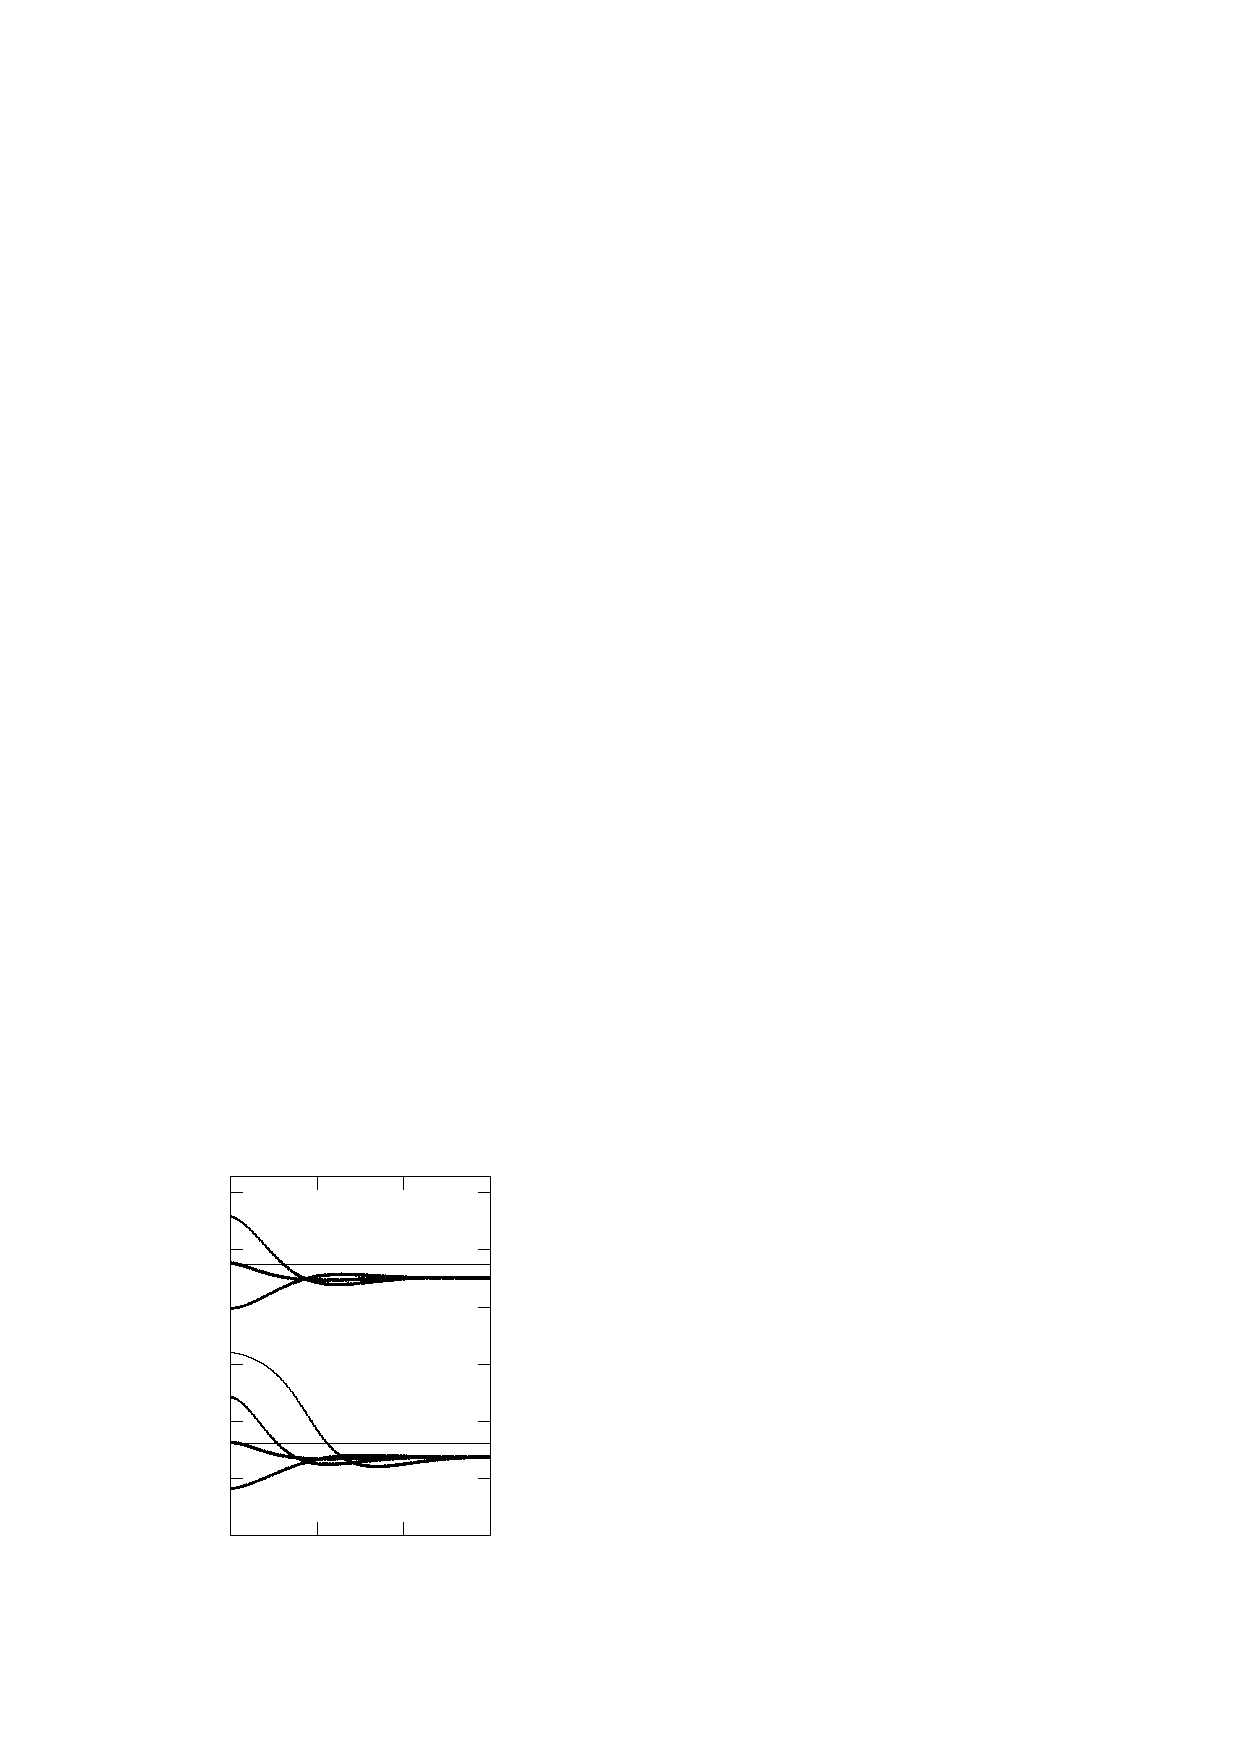
\includegraphics{eps/position-flat-nonzerogravity}%
\end{picture}%
\begingroup
\setlength{\unitlength}{0.0200bp}%
\begin{picture}(9000,10800)(0,0)%
\put(1650,1650){\makebox(0,0)[r]{\strut{} 0}}%
\put(1650,3019){\makebox(0,0)[r]{\strut{} 1}}%
\put(1650,4389){\makebox(0,0)[r]{\strut{} 2}}%
\put(1650,5758){\makebox(0,0)[r]{\strut{} 3}}%
\put(1650,7128){\makebox(0,0)[r]{\strut{} 4}}%
\put(1650,8497){\makebox(0,0)[r]{\strut{} 5}}%
\put(1650,9867){\makebox(0,0)[r]{\strut{} 6}}%
\put(1925,1100){\makebox(0,0){\strut{} 0}}%
\put(4008,1100){\makebox(0,0){\strut{} 60}}%
\put(6092,1100){\makebox(0,0){\strut{} 120}}%
\put(8175,1100){\makebox(0,0){\strut{} 180}}%
\put(550,5950){\rotatebox{90}{\makebox(0,0){\strut{}$y^\ast$}}}%
\put(5050,275){\makebox(0,0){\strut{}$t^\ast$}}%

\put(7650,9588){\makebox(0,0)[r]{\strut{} (a)}}%
\end{picture}%
\endgroup
\endinput

%GNUPLOT: LaTeX picture with Postscript
\begin{picture}(0,0)%
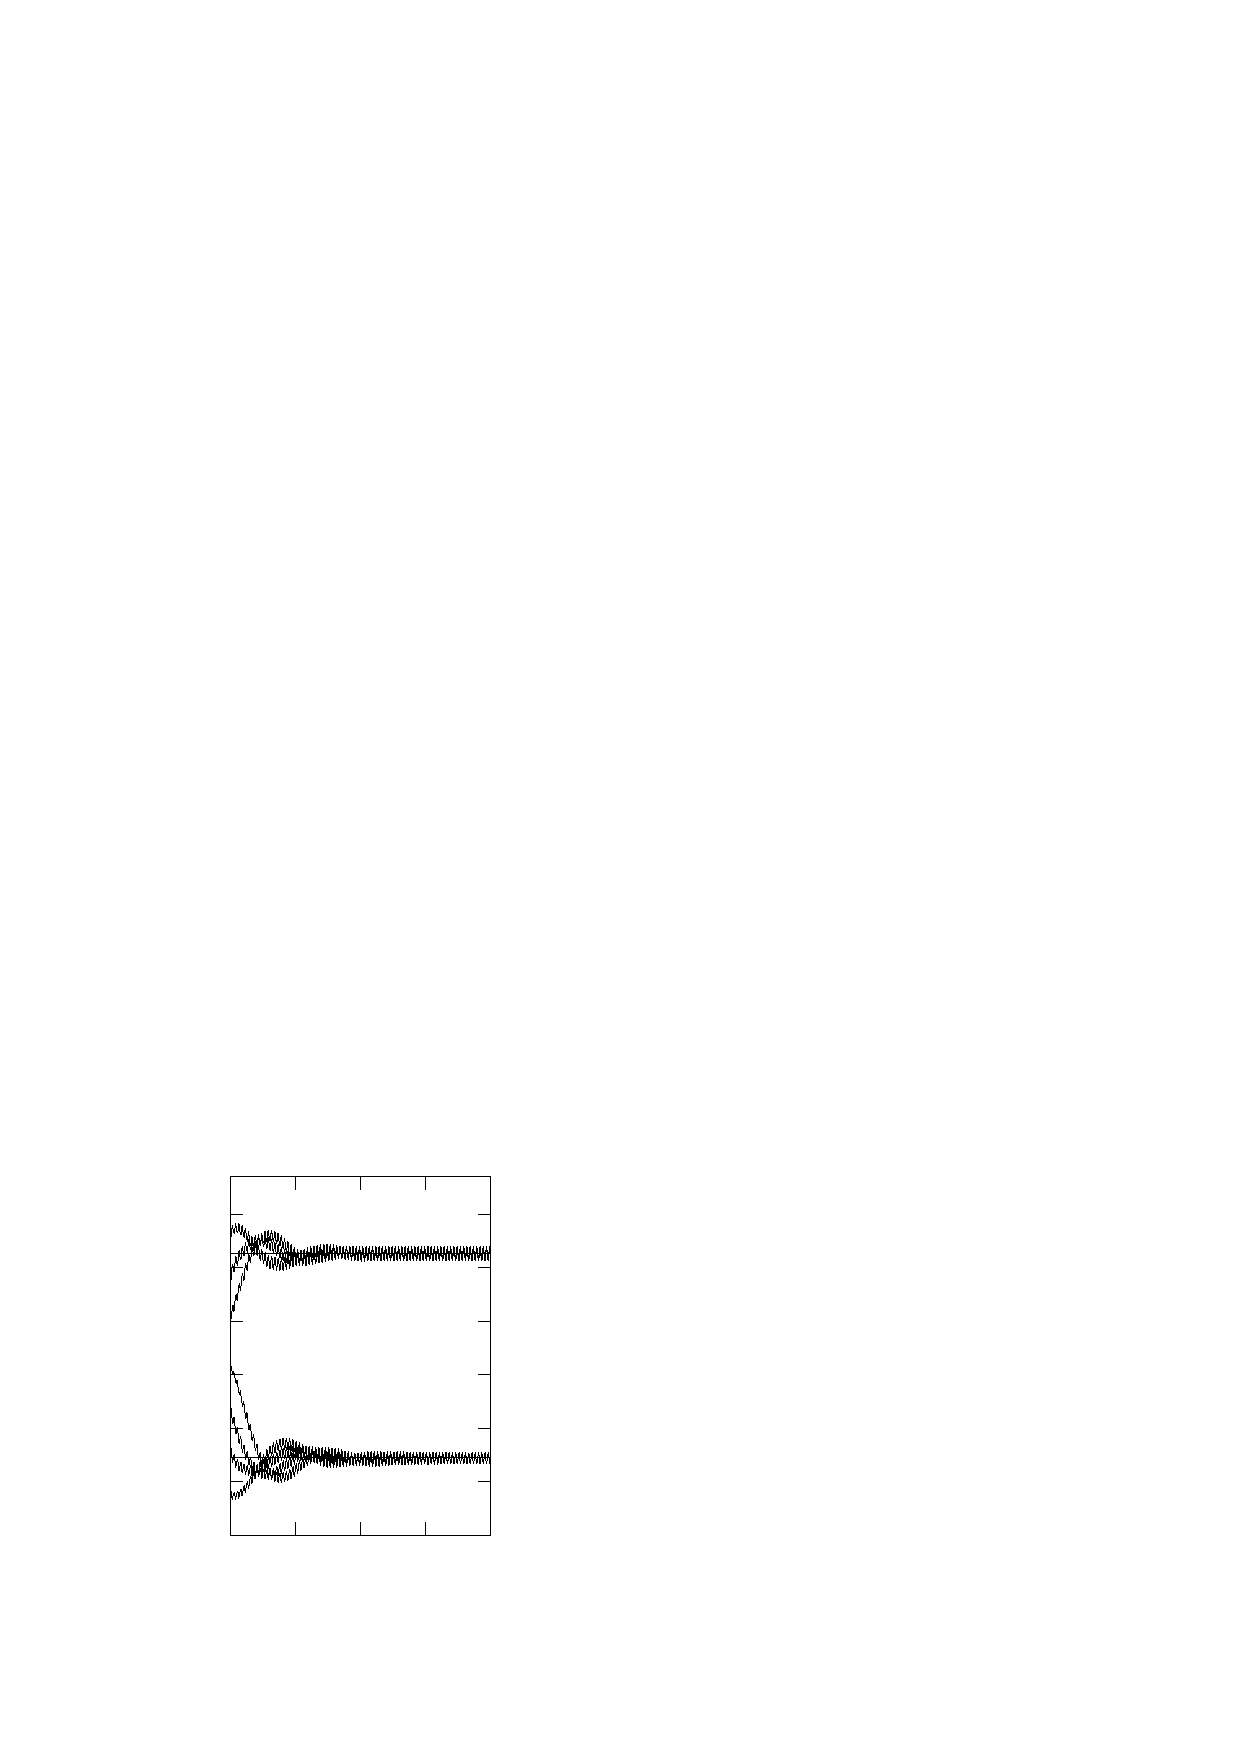
\includegraphics{eps/position-rounded-nonzerogravity}%
\end{picture}%
\begingroup
\setlength{\unitlength}{0.0200bp}%
\begin{picture}(9000,10800)(0,0)%
\put(1650,1650){\makebox(0,0)[r]{\strut{} 0}}%
\put(1650,2934){\makebox(0,0)[r]{\strut{} 1}}%
\put(1650,4217){\makebox(0,0)[r]{\strut{} 2}}%
\put(1650,5501){\makebox(0,0)[r]{\strut{} 3}}%
\put(1650,6784){\makebox(0,0)[r]{\strut{} 4}}%
\put(1650,8068){\makebox(0,0)[r]{\strut{} 5}}%
\put(1650,9351){\makebox(0,0)[r]{\strut{} 6}}%
\put(1925,1100){\makebox(0,0){\strut{} 0}}%
\put(3488,1100){\makebox(0,0){\strut{} 20}}%
\put(5050,1100){\makebox(0,0){\strut{} 40}}%
\put(6613,1100){\makebox(0,0){\strut{} 60}}%
\put(8175,1100){\makebox(0,0){\strut{} 80}}%
\put(550,5950){\rotatebox{90}{\makebox(0,0){\strut{}$y^\ast$}}}%
\put(5050,275){\makebox(0,0){\strut{}$t^\ast$}}%

\put(7650,9588){\makebox(0,0)[r]{\strut{} (b)}}%

\end{picture}%
\endgroup
\endinput

\vskip 5mm
\caption{\label{fig:path-3}
 Vertical positions of particles with $r^\ast=0.25$ and twice the 
 density of the fluid in the presence of gravity for (a) the flat cavity and (b) the 
 rounded one. The horizontal lines represent the vertical position of the pressure node. 
 The oscillations in the flat cavity are barely visible. 
 For both cavities $P_o^\ast = 1.6\times 10^{-3}$. Lattices of $163\times 201$ and 
 $901\times 251$ nodes were used for the flat and rounded cavity respectively.}
\end{figure}

In the following, we report the results of numerical simulations in the second
resonant mode with the particle initially near the pressure node closest to the reflector.
In Figs.~\ref{fig:barrido-rho} (a) and (b) we show  $y_s^\ast$, the time average of 
the vertical position of the particle after a long transient, as the ratio of
the density of the particle $\rho_p$ and the fluid $\rho_f$
varies for a fixed value of $P_o^\ast$. We also show the standard 
deviation which is a measure of the amplitude of oscillation of the particle around 
$y_s^\ast$. There is a near linear behaviour in both cavities which implies that the 
mean acoustical force is proportional to the deviation of $y_s^\ast$ from the 
pressure node. A detailed analysis of all trajectories indicates the presence of a 
small amplitude oscillation with frequency $\omega_o$ and its harmonics. The large 
values of the standard deviation of $y_s^\ast$ in the rounded cavity for 
$50\lsim\rho_p/\rho_f\lsim 250$ are the consequence of large amplitude oscillations of 
frequency $\omega_1$ and its harmonics with $\omega_1\ll\omega_o$. 
%
\begin{figure}
%GNUPLOT: LaTeX picture with Postscript
\begin{picture}(0,0)%
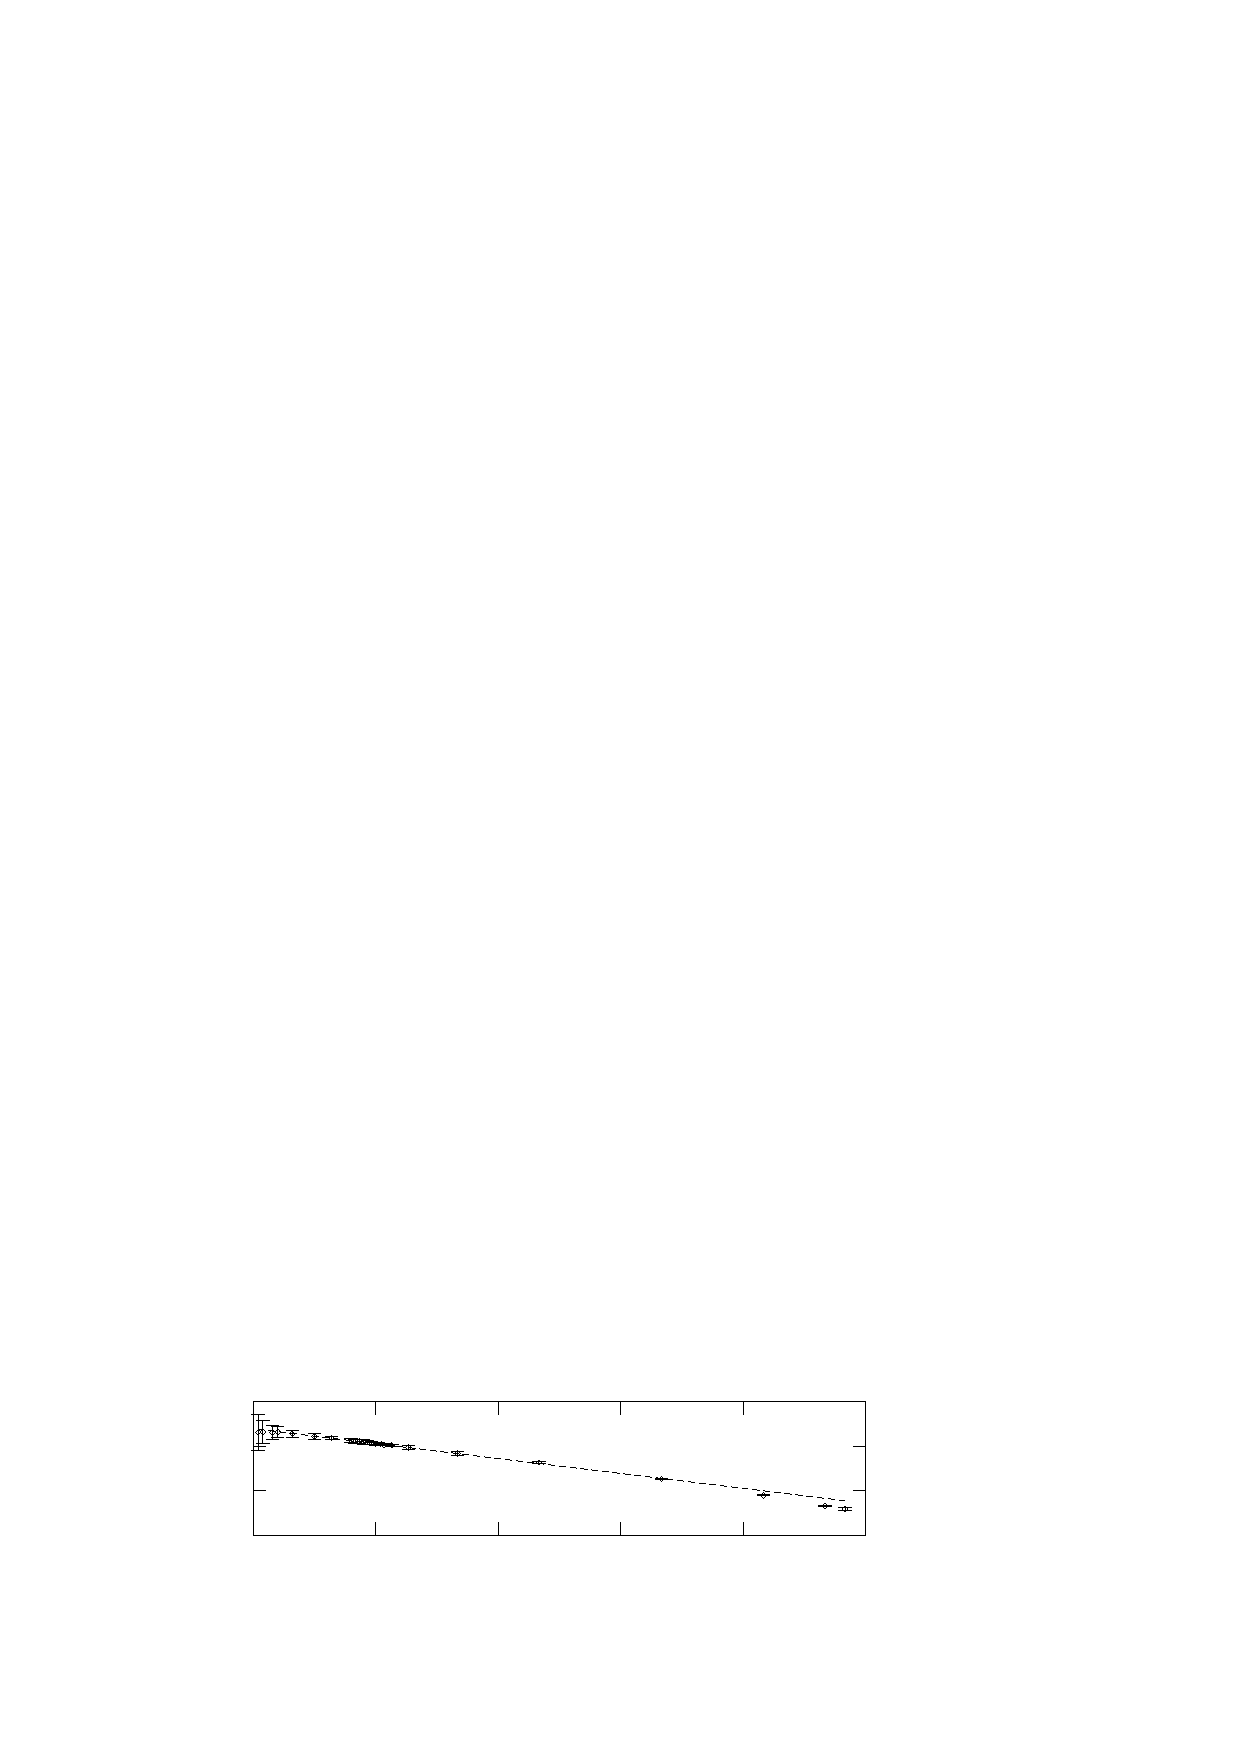
\includegraphics{barrido-rho-flat-ajuste}%
\end{picture}%
\begingroup
\setlength{\unitlength}{0.0200bp}%
\begin{picture}(18000,5400)(0,0)%
\put(2200,1650){\makebox(0,0)[r]{\strut{}1.00}}%
\put(2200,2717){\makebox(0,0)[r]{\strut{}1.25}}%
\put(2200,3783){\makebox(0,0)[r]{\strut{}1.50}}%
\put(2200,4850){\makebox(0,0)[r]{\strut{}1.75}}%
\put(2475,1100){\makebox(0,0){\strut{} 0}}%
\put(5415,1100){\makebox(0,0){\strut{} 50}}%
\put(8355,1100){\makebox(0,0){\strut{} 100}}%
\put(11295,1100){\makebox(0,0){\strut{} 150}}%
\put(14235,1100){\makebox(0,0){\strut{} 200}}%
\put(17175,1100){\makebox(0,0){\strut{} 250}}%
\put(550,3250){\rotatebox{90}{\makebox(0,0){\strut{}$y^\ast_{es}$}}}%
\put(9825,275){\makebox(0,0){\strut{}$\rho_p/\rho_f$}}%
\put(600,1000){\rotatebox{0}{\makebox(0,0){\strut{}(a)}}}%
\end{picture}%
\endgroup
\endinput

%GNUPLOT: LaTeX picture with Postscript
\begin{picture}(0,0)%
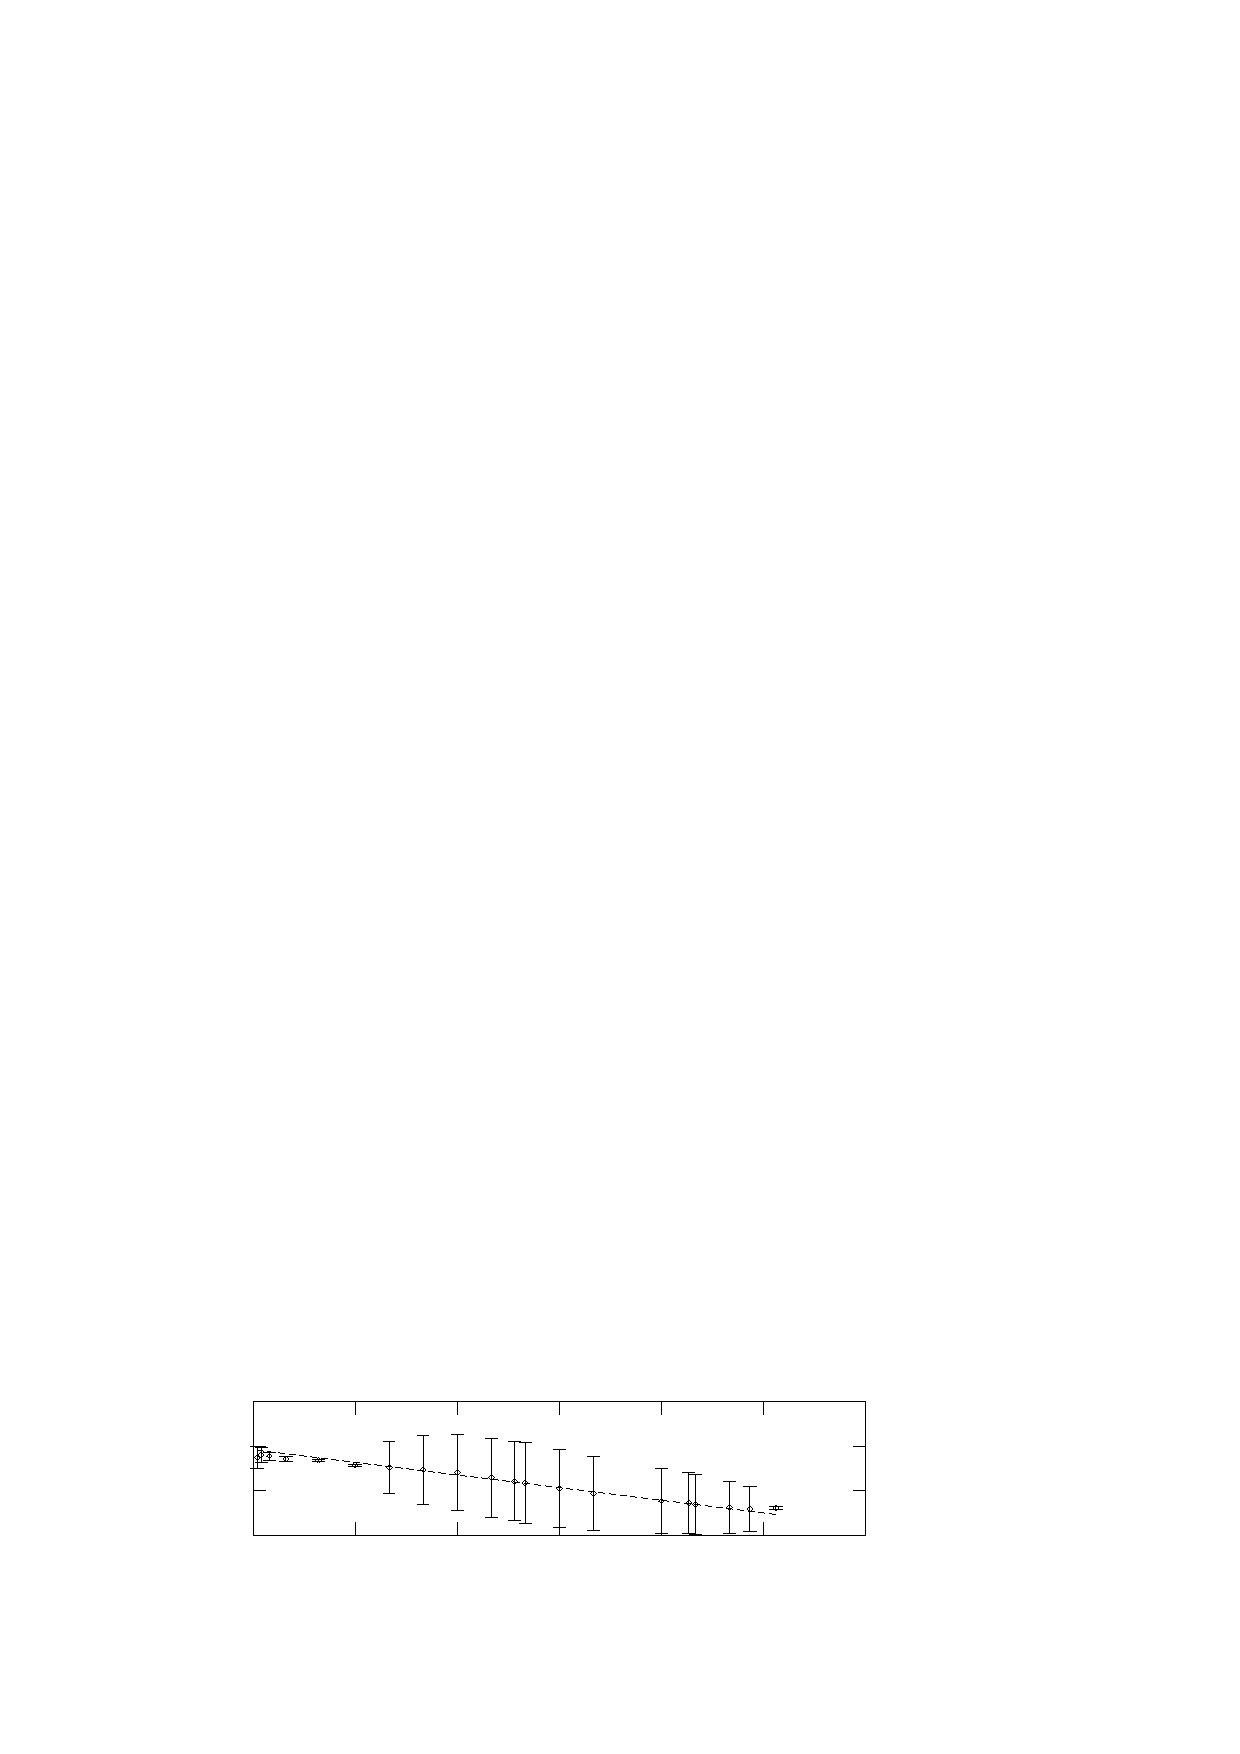
\includegraphics{barrido-rho-rounded-ajuste}%
\end{picture}%
\begingroup
\setlength{\unitlength}{0.0200bp}%
\begin{picture}(18000,5400)(0,0)%
\put(2200,1650){\makebox(0,0)[r]{\strut{}0.80}}%
\put(2200,2717){\makebox(0,0)[r]{\strut{}1.20}}%
\put(2200,3783){\makebox(0,0)[r]{\strut{}1.60}}%
\put(2200,4850){\makebox(0,0)[r]{\strut{}2.00}}%
\put(2475,1100){\makebox(0,0){\strut{} 0}}%
\put(4925,1100){\makebox(0,0){\strut{} 50}}%
\put(7375,1100){\makebox(0,0){\strut{} 100}}%
\put(9825,1100){\makebox(0,0){\strut{} 150}}%
\put(12275,1100){\makebox(0,0){\strut{} 200}}%
\put(14725,1100){\makebox(0,0){\strut{} 250}}%
\put(17175,1100){\makebox(0,0){\strut{} 300}}%
\put(550,3250){\rotatebox{90}{\makebox(0,0){\strut{}$y_{es}^\ast$}}}%
\put(9825,275){\makebox(0,0){\strut{}$\rho_p/\rho_f$}}%
\put(600,1000){\rotatebox{0}{\makebox(0,0){\strut{}(b)}}}%
\end{picture}%
\endgroup
\endinput

\caption{\label{fig:barrido-rho}
 Vertical stationary position $y_s^\ast$ with its standard deviation as $\rho_p/\rho_f$ 
 varies for (a) the flat and (b) the rounded cavity. In the numerical simulations 
 $P^\ast=0.01$ for the flat cavity and $P^\ast=0.0019$ for the rounded one. The slopes 
 of the linear fit are (a) $-0.00168$ and (b) $-0.00227$. 
}
\end{figure}

In Figs.~\ref{fig:barrido-momento} (a) and (b) we show $y_s^\ast$ with its standard 
deviation as $P_o^\ast$, the amplitude of the applied external momentum varies, 
keeping $\rho_p/\rho_f$ fixed. As $P_o^\ast$ grows, $y_s^\ast$ approaches the pressure 
node in the flat cavity. For the rounded cavity, the situation is more complex, since 
the pressure node's position depends on $P_o^\ast$ as we also show in 
Fig.~\ref{fig:barrido-momento} (b). In order to begin to explain the results found for 
the rounded cavity we show the vertical positions for three values of $P_o^\ast$ in 
Figs.~\ref{fig:paths-rho-30-rounded}. In Figs.~\ref{fig:paths-rho-30-rounded} (a) and (b) 
there is a small amplitude oscillation with frequency $\omega_o$ and its harmonics, while 
in Fig.~\ref{fig:paths-rho-30-rounded} (c) this oscillation has been filtered out. In 
Fig.~\ref{fig:paths-rho-30-rounded} (a), that corresponds to the smallest value of 
$P_o^\ast$ in Fig.~\ref{fig:barrido-momento} (b), the power spectrum shows a second
frequency $\omega_1$, much smaller than $\omega_o$, together with its harmonics.
These low frequency oscillations are present in all the numerical simulations reported
in Fig.~\ref{fig:barrido-momento} (b) except the one for the largest value of $P_o^\ast$.
In Fig.~\ref{fig:paths-rho-30-rounded} (b), for $P_o^\ast$ where the standard deviation 
of $y_s^\ast$ in Fig.~\ref{fig:barrido-momento} (b) begins to grow, and (c), for the last 
value of $P_o^\ast$ in that Fig.~the oscillations  are more complex. The origin of this 
change is in the horizontal motion of the particle which was not present before due to a 
doubling of the pressure node nearest the rounded reflector for $P_o^\ast>P_{o_c}^\ast$ 
with $P_{o_c}^\ast$ between 0.0032 and 0.0038 as we show in 
Fig.~\ref{fig:bifurcacion-rounded}. For $P_o^\ast>P_{o_c}^\ast$, except for the last
value of $P_o^\ast$ shown in Fig.~\ref{fig:barrido-momento} (b) the particle oscillates
horizontally with frequencies $\omega_o$ and and its harmonics and a much smaller
frequency $\omega_2$ and its harmonics.
%
\begin{figure}
%GNUPLOT: LaTeX picture with Postscript
\begin{picture}(0,0)%
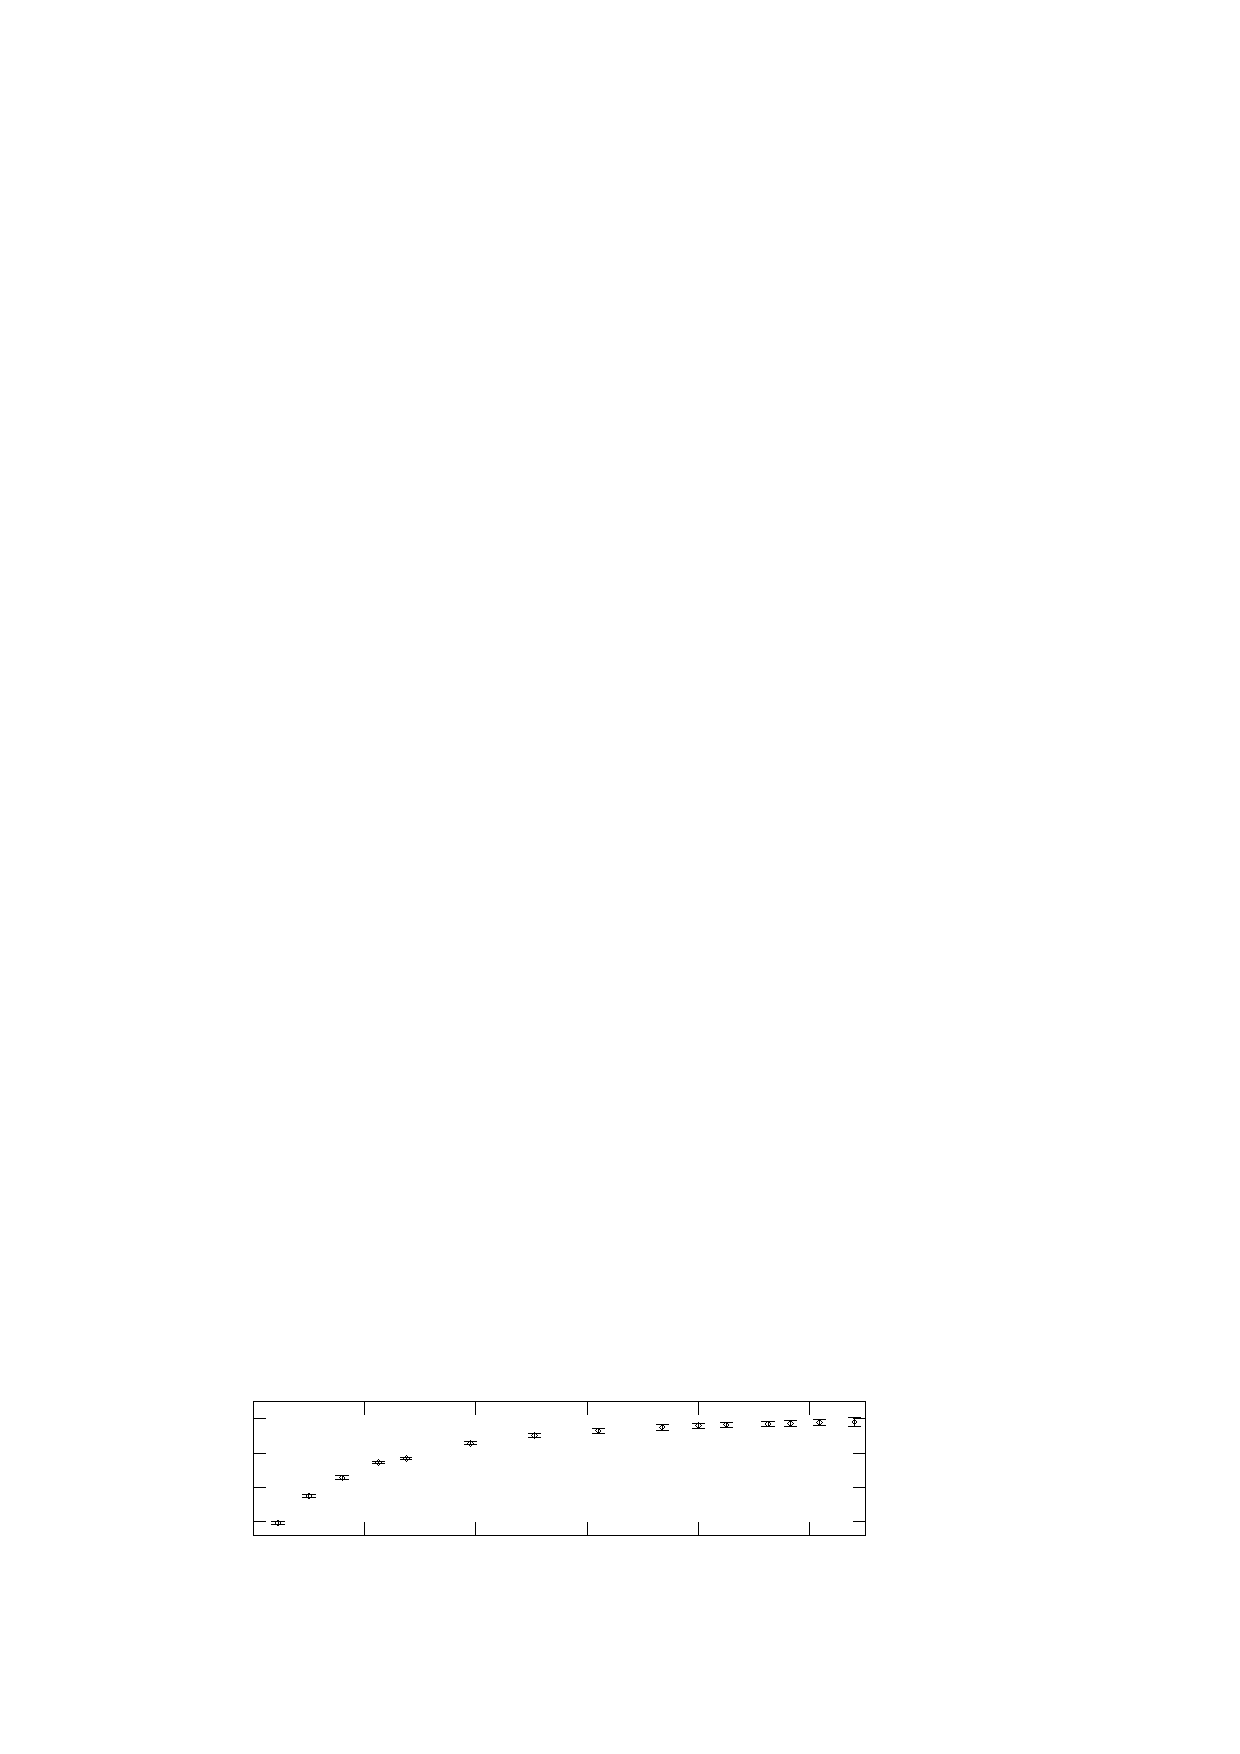
\includegraphics{Fo-equilibrium-amplitud-flat}%
\end{picture}%
\begingroup
\setlength{\unitlength}{0.0200bp}%
\begin{picture}(18000,5400)(0,0)%
\put(2200,1990){\makebox(0,0)[r]{\strut{}1.20}}%
\put(2200,2807){\makebox(0,0)[r]{\strut{}1.32}}%
\put(2200,3624){\makebox(0,0)[r]{\strut{}1.44}}%
\put(2200,4441){\makebox(0,0)[r]{\strut{}1.56}}%
\put(2475,1100){\makebox(0,0){\strut{}0.004}}%
\put(5148,1100){\makebox(0,0){\strut{}0.006}}%
\put(7820,1100){\makebox(0,0){\strut{}0.008}}%
\put(10493,1100){\makebox(0,0){\strut{}0.010}}%
\put(13166,1100){\makebox(0,0){\strut{}0.012}}%
\put(15839,1100){\makebox(0,0){\strut{}0.014}}%
\put(550,3250){\rotatebox{90}{\makebox(0,0){\strut{}$y_{s}^\ast$}}}%
\put(9825,275){\makebox(0,0){\strut{}$P_o^\ast$}}%
\put(3800,4350){\makebox(0,0)[r]{\strut{}(a)}}%
\end{picture}%
\endgroup
\endinput

%GNUPLOT: LaTeX picture with Postscript
\begin{picture}(0,0)%
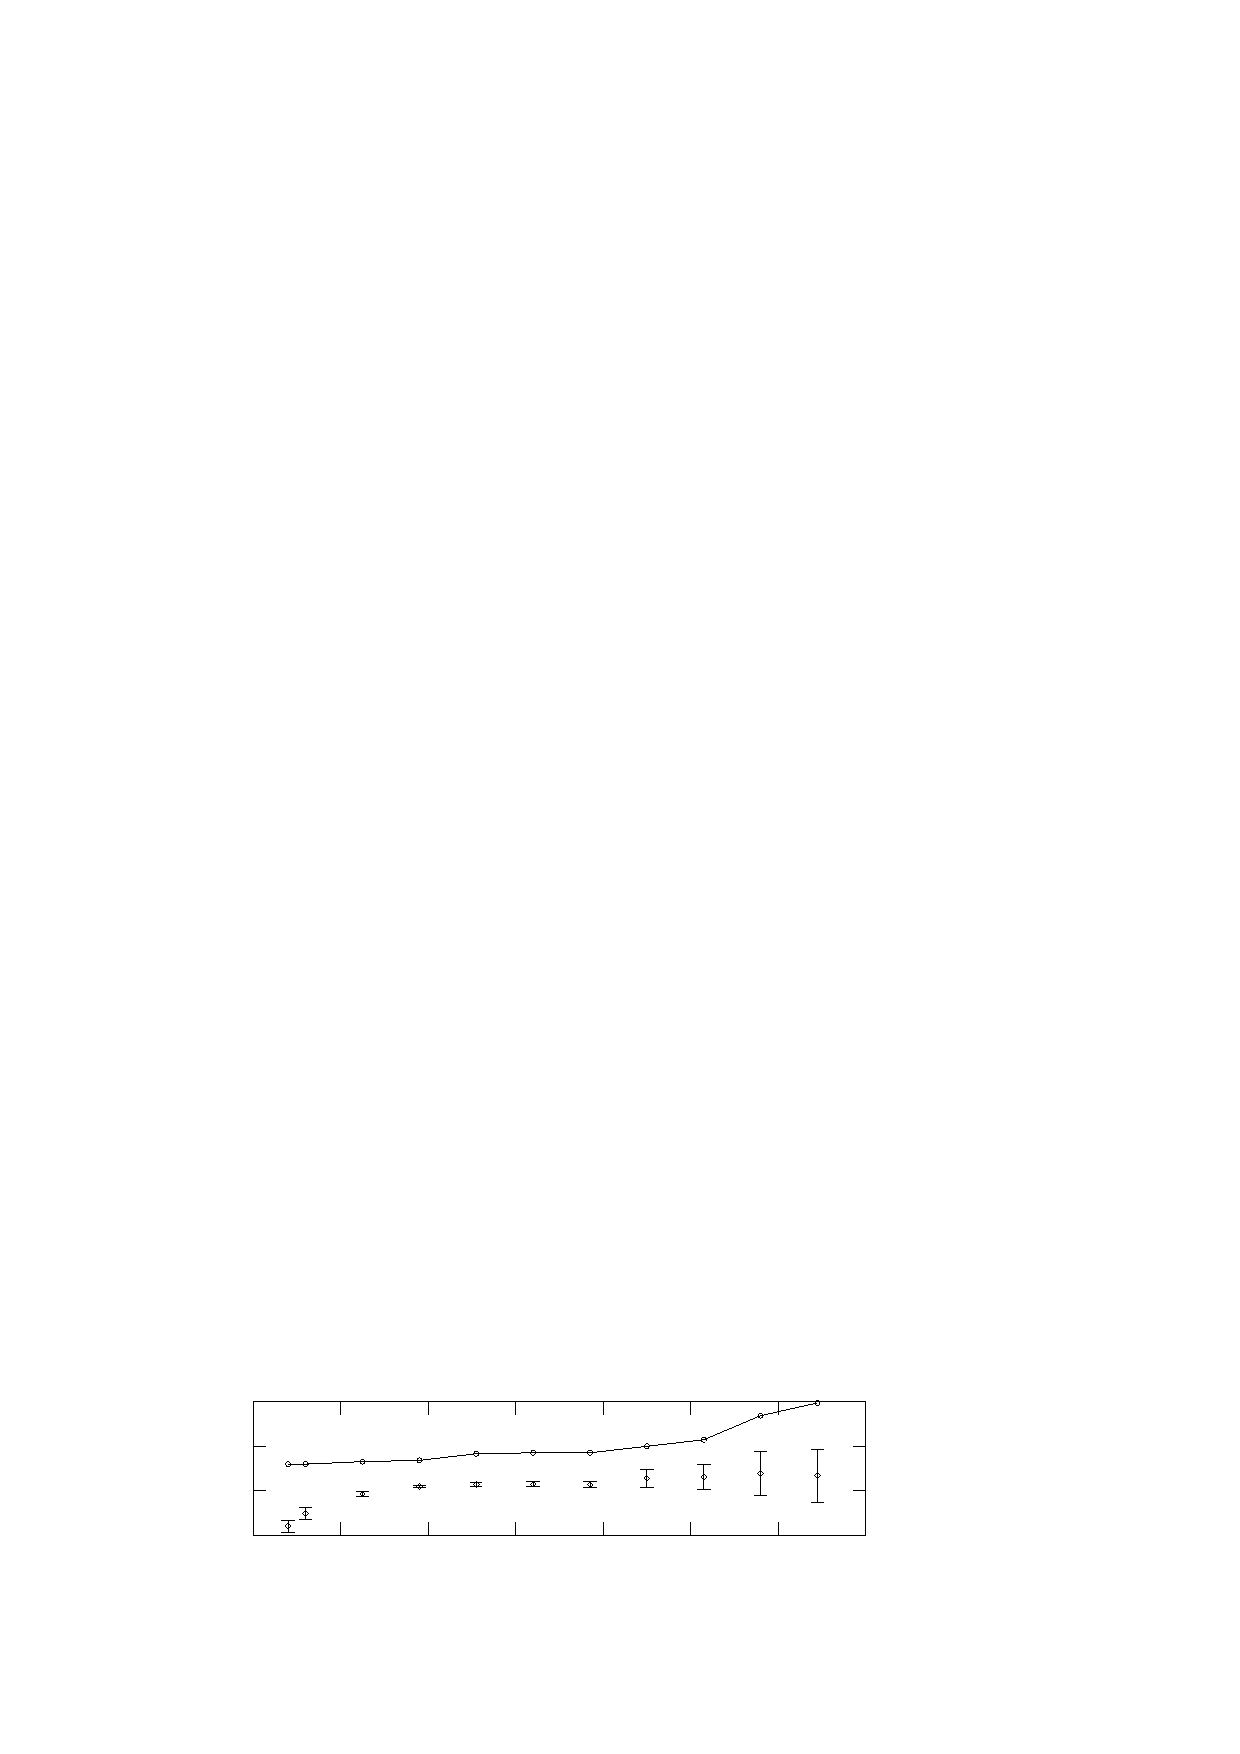
\includegraphics{Fo-equilibrium-amplitud-rounded}%
\end{picture}%
\begingroup
\setlength{\unitlength}{0.0200bp}%
\begin{picture}(18000,5400)(0,0)%
\put(2200,1650){\makebox(0,0)[r]{\strut{}1.05}}%
\put(2200,2717){\makebox(0,0)[r]{\strut{}1.40}}%
\put(2200,3783){\makebox(0,0)[r]{\strut{}1.75}}%
\put(2200,4850){\makebox(0,0)[r]{\strut{}2.10}}%
\put(2475,1100){\makebox(0,0){\strut{}0.000}}%
\put(4575,1100){\makebox(0,0){\strut{}0.001}}%
\put(6675,1100){\makebox(0,0){\strut{}0.002}}%
\put(8775,1100){\makebox(0,0){\strut{}0.003}}%
\put(10875,1100){\makebox(0,0){\strut{}0.004}}%
\put(12975,1100){\makebox(0,0){\strut{}0.005}}%
\put(15075,1100){\makebox(0,0){\strut{}0.006}}%
\put(17175,1100){\makebox(0,0){\strut{}0.007}}%
\put(550,3250){\rotatebox{90}{\makebox(0,0){\strut{}$y_s^\ast$}}}%
\put(9825,275){\makebox(0,0){\strut{}$P^\ast_o$}}%
\put(3800,4350){\makebox(0,0)[r]{\strut{}(b)}}%
\end{picture}%
\endgroup
\endinput

\caption{\label{fig:barrido-momento}
 Vertical stationary position $y_s^\ast$ with its standard deviation as 
 $P_o^\ast$ varies with $\rho_p/\rho_f=50$ for the (a) flat and (b) rounded 
 cavities. In the flat cavity, the pressure node is at $y^\ast=1.6$. The curve in (b) 
 shows the vertical position of the pressure node.
}
\end{figure}
%
\begin{figure}
%GNUPLOT: LaTeX picture with Postscript
\begin{picture}(0,0)%
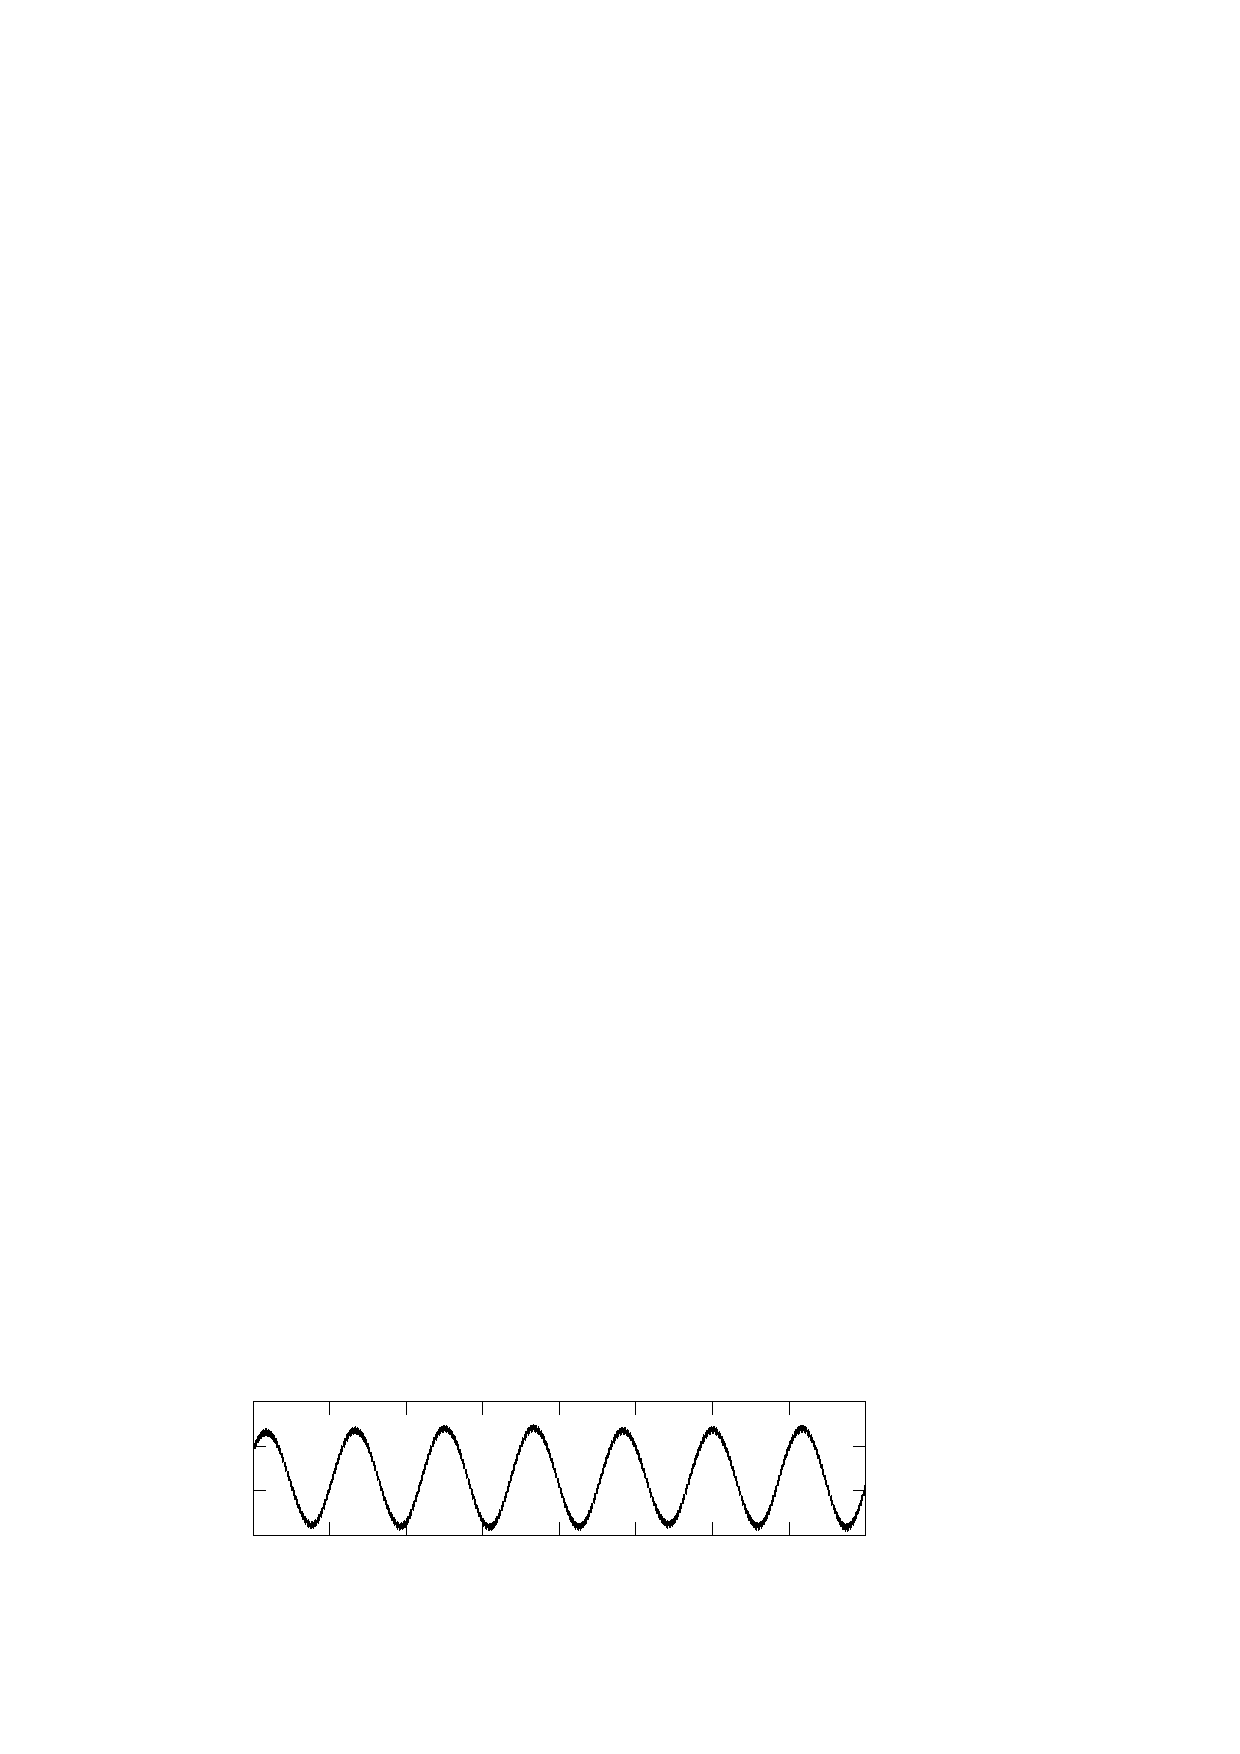
\includegraphics{rounded-rhop30-Fo7_508e-03}%
\end{picture}%
\begingroup
\setlength{\unitlength}{0.0200bp}%
\begin{picture}(18000,5400)(0,0)%
\put(2200,1650){\makebox(0,0)[r]{\strut{}1.14}}%
\put(2200,2717){\makebox(0,0)[r]{\strut{}1.20}}%
\put(2200,3783){\makebox(0,0)[r]{\strut{}1.26}}%
\put(2200,4850){\makebox(0,0)[r]{\strut{}1.32}}%
\put(2475,1100){\makebox(0,0){\strut{} 1600}}%
\put(4313,1100){\makebox(0,0){\strut{} 1650}}%
\put(6150,1100){\makebox(0,0){\strut{} 1700}}%
\put(7988,1100){\makebox(0,0){\strut{} 1750}}%
\put(9825,1100){\makebox(0,0){\strut{} 1800}}%
\put(11663,1100){\makebox(0,0){\strut{} 1850}}%
\put(13500,1100){\makebox(0,0){\strut{} 1900}}%
\put(15338,1100){\makebox(0,0){\strut{} 1950}}%
\put(17175,1100){\makebox(0,0){\strut{} 2000}}%
\put(550,3250){\rotatebox{90}{\makebox(0,0){\strut{}$y^\ast$}}}%
\put(9825,275){\makebox(0,0){\strut{}$t^\ast$}}%
\put(600,1000){\rotatebox{0}{\makebox(0,0){\strut{}(a)}}}%
\end{picture}%
\endgroup
\endinput

%GNUPLOT: LaTeX picture with Postscript
\begin{picture}(0,0)%
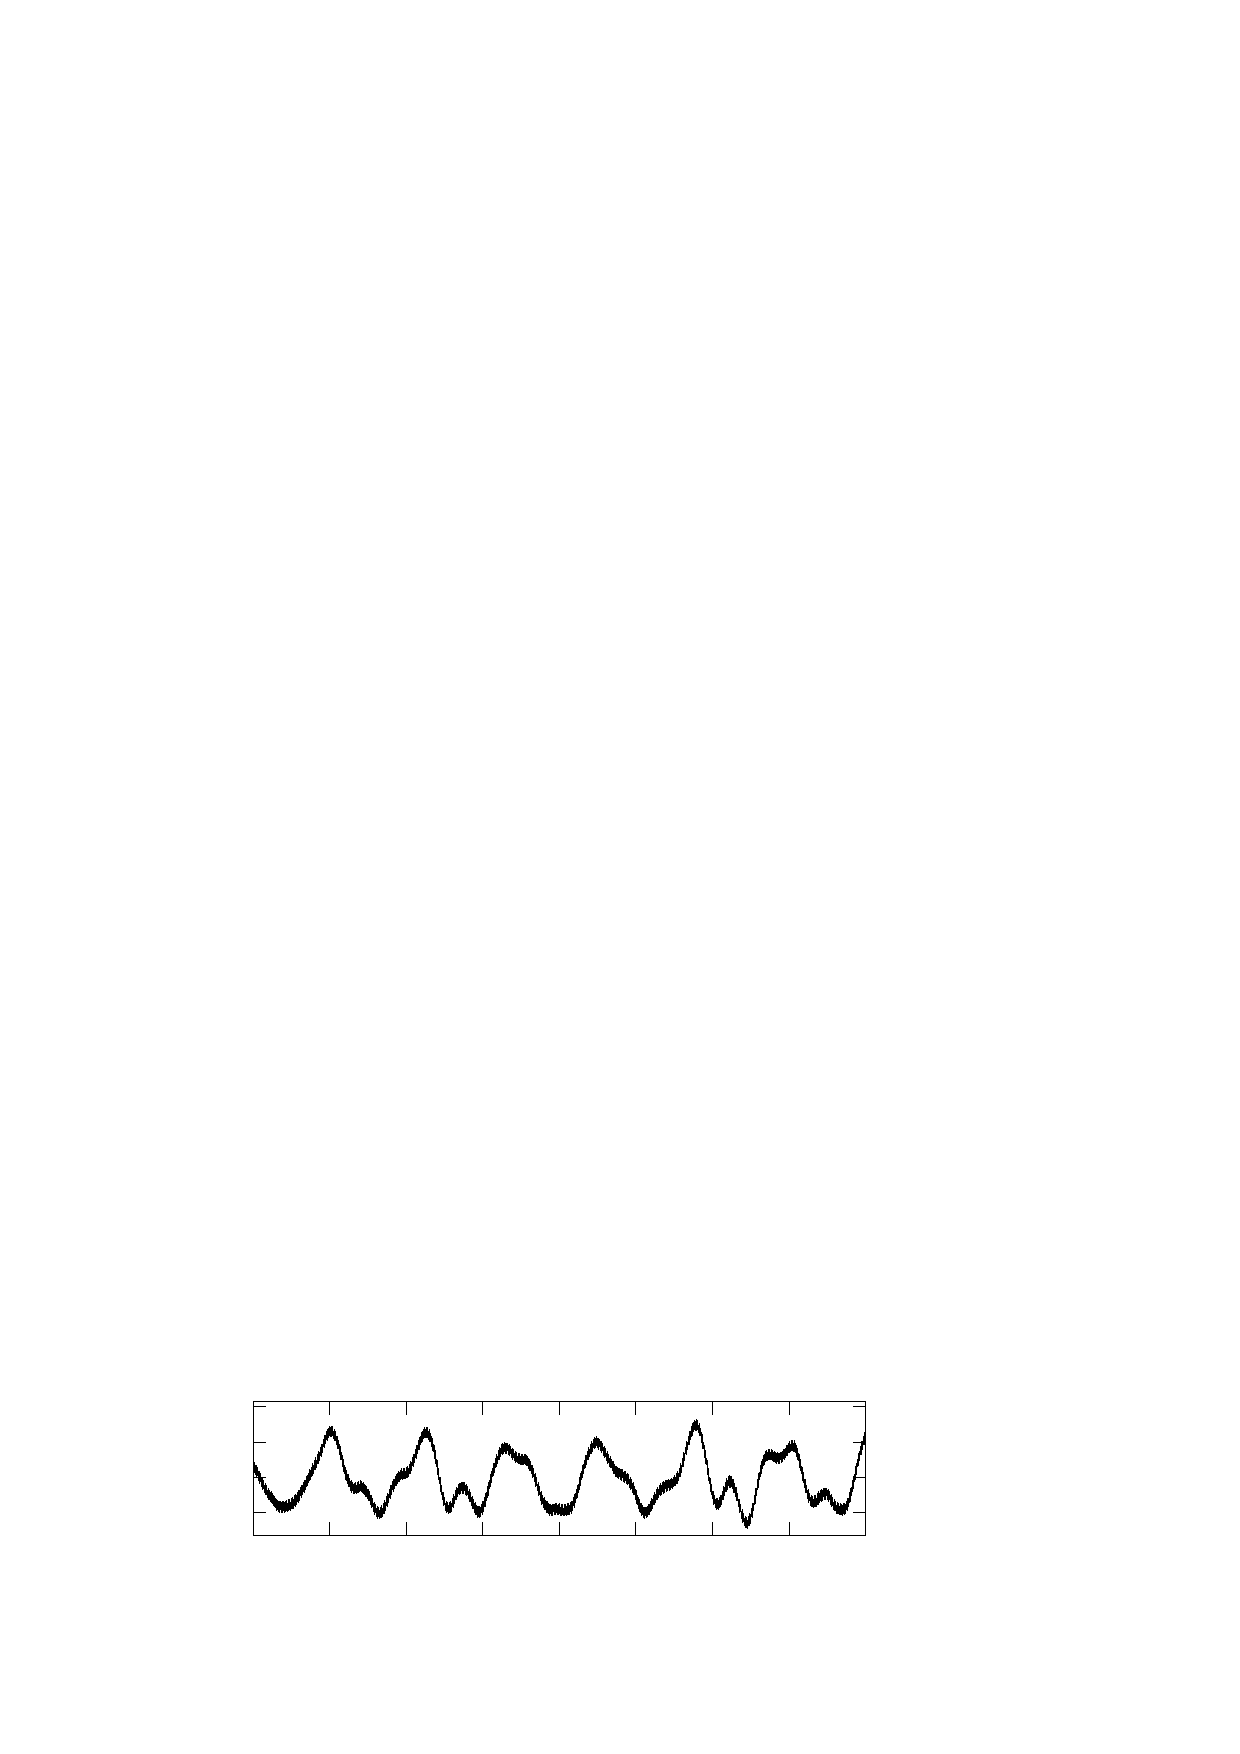
\includegraphics{rounded-rhop30-Fo5_631e-02}%
\end{picture}%
\begingroup
\setlength{\unitlength}{0.0200bp}%
\begin{picture}(18000,5400)(0,0)%
\put(2200,2193){\makebox(0,0)[r]{\strut{}1.40}}%
\put(2200,3040){\makebox(0,0)[r]{\strut{}1.50}}%
\put(2200,3887){\makebox(0,0)[r]{\strut{}1.60}}%
\put(2200,4734){\makebox(0,0)[r]{\strut{}1.70}}%
\put(2475,1100){\makebox(0,0){\strut{} 1600}}%
\put(4313,1100){\makebox(0,0){\strut{} 1650}}%
\put(6150,1100){\makebox(0,0){\strut{} 1700}}%
\put(7988,1100){\makebox(0,0){\strut{} 1750}}%
\put(9825,1100){\makebox(0,0){\strut{} 1800}}%
\put(11663,1100){\makebox(0,0){\strut{} 1850}}%
\put(13500,1100){\makebox(0,0){\strut{} 1900}}%
\put(15338,1100){\makebox(0,0){\strut{} 1950}}%
\put(17175,1100){\makebox(0,0){\strut{} 2000}}%
\put(550,3250){\rotatebox{90}{\makebox(0,0){\strut{}$y^\ast$}}}%
\put(9825,275){\makebox(0,0){\strut{}$t^\ast$}}%
\put(600,1000){\rotatebox{0}{\makebox(0,0){\strut{}(b)}}}%
\end{picture}%
\endgroup
\endinput

%GNUPLOT: LaTeX picture with Postscript
\begin{picture}(0,0)%
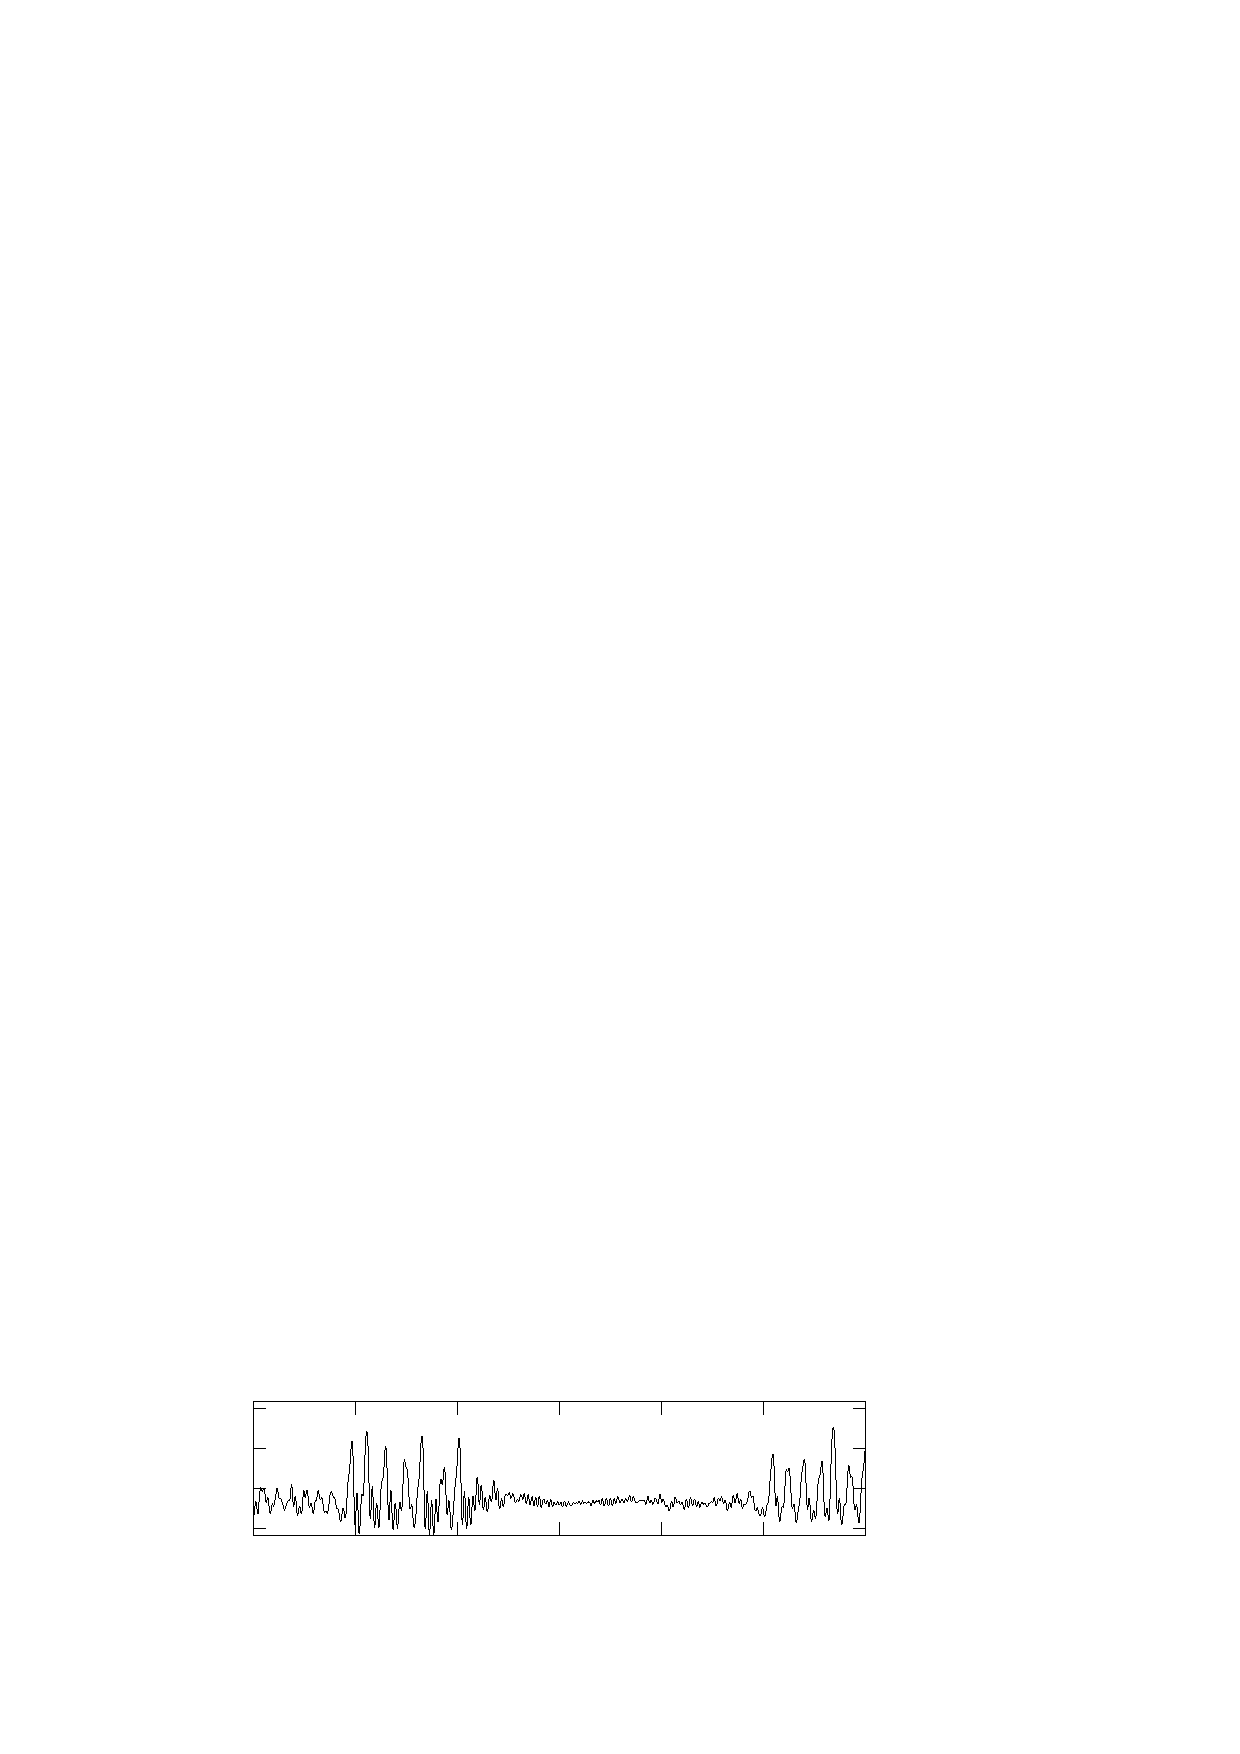
\includegraphics{rounded-rhop30-Fo8_072e-02}%
\end{picture}%
\begingroup
\setlength{\unitlength}{0.0200bp}%
\begin{picture}(18000,5400)(0,0)%
\put(2200,1805){\makebox(0,0)[r]{\strut{}1.20}}%
\put(2200,2765){\makebox(0,0)[r]{\strut{}1.60}}%
\put(2200,3725){\makebox(0,0)[r]{\strut{}2.00}}%
\put(2200,4685){\makebox(0,0)[r]{\strut{}2.40}}%
\put(2475,1100){\makebox(0,0){\strut{} 500}}%
\put(4925,1100){\makebox(0,0){\strut{} 1000}}%
\put(7375,1100){\makebox(0,0){\strut{} 1500}}%
\put(9825,1100){\makebox(0,0){\strut{} 2000}}%
\put(12275,1100){\makebox(0,0){\strut{} 2500}}%
\put(14725,1100){\makebox(0,0){\strut{} 3000}}%
\put(17175,1100){\makebox(0,0){\strut{} 3500}}%
\put(550,3250){\rotatebox{90}{\makebox(0,0){\strut{}$y^\ast$}}}%
\put(9825,275){\makebox(0,0){\strut{}$t^\ast$}}%
\put(600,1000){\rotatebox{0}{\makebox(0,0){\strut{}(c)}}}%
\end{picture}%
\endgroup
\endinput

%GNUPLOT: LaTeX picture with Postscript
\begin{picture}(0,0)%
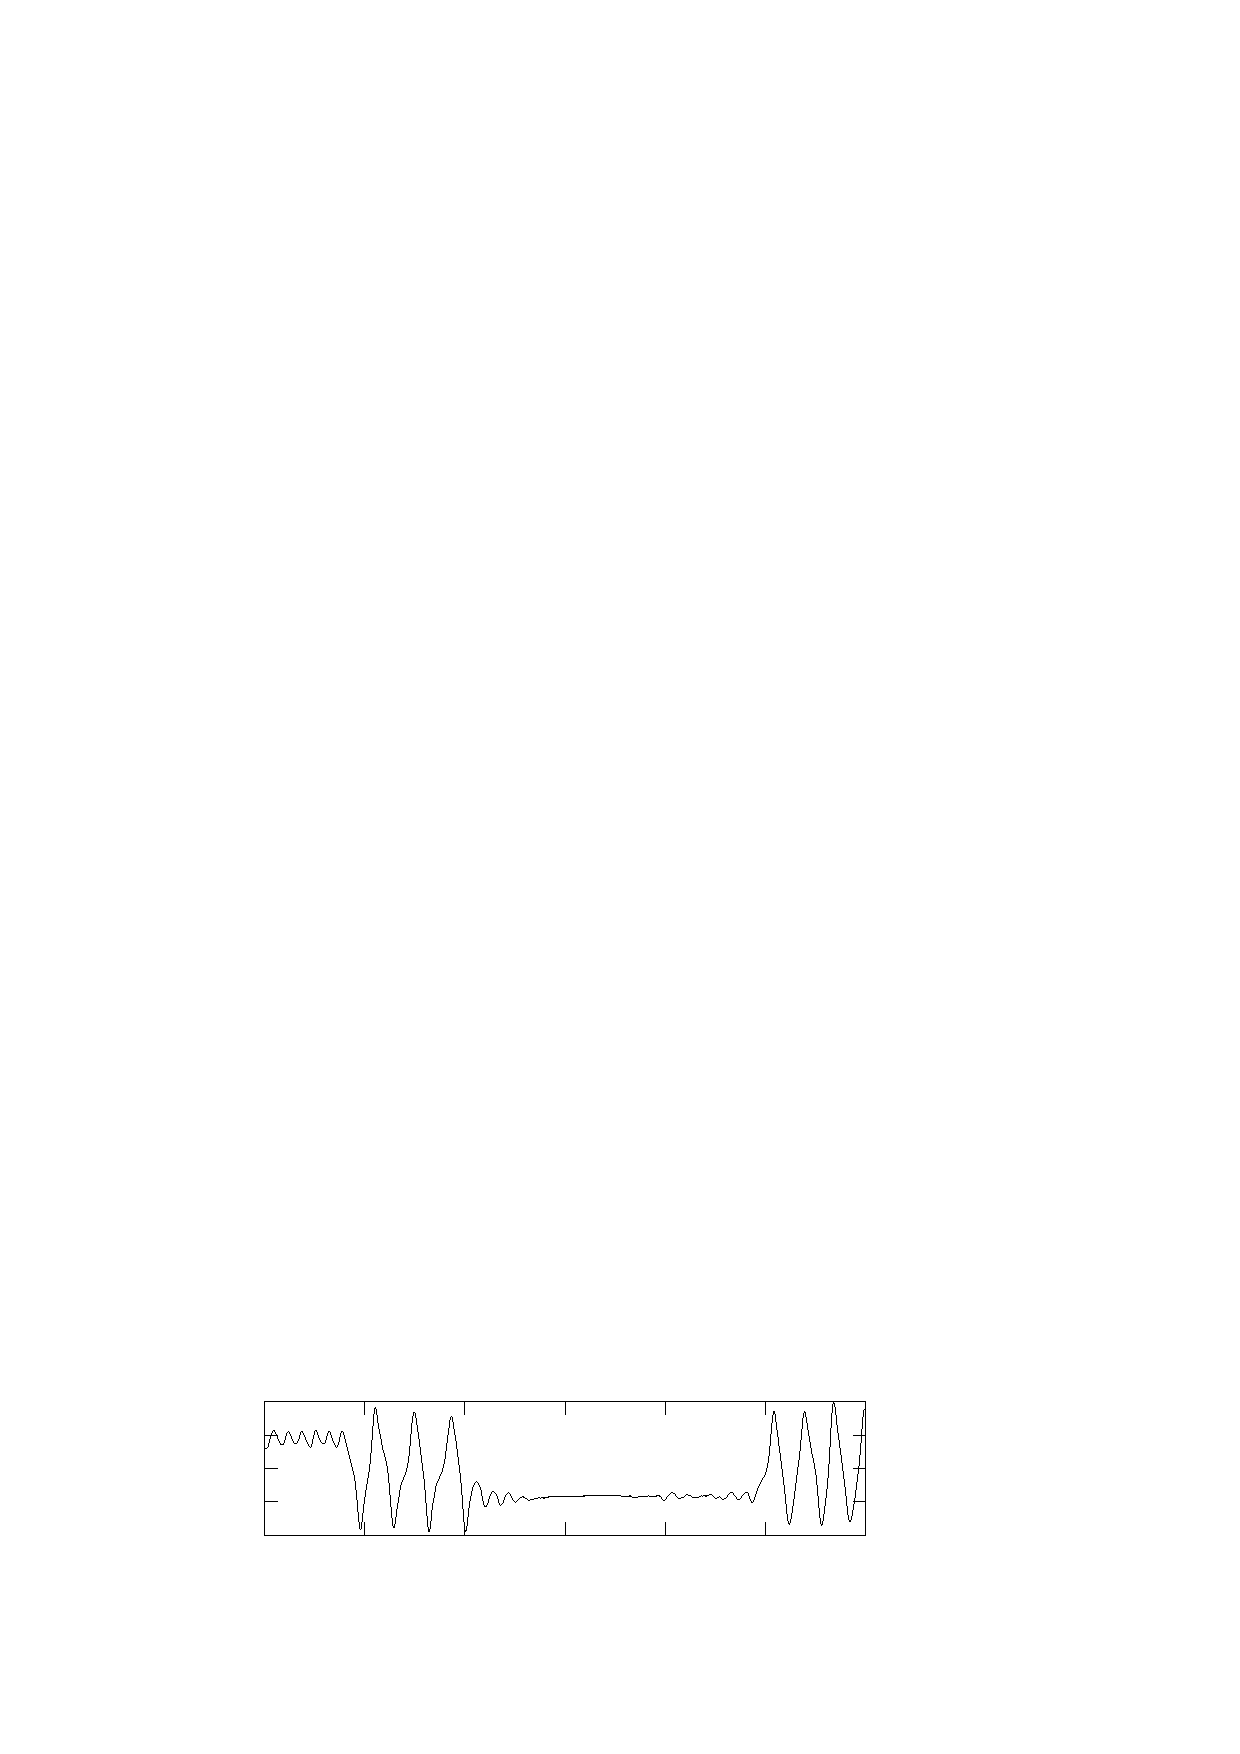
\includegraphics{rounded-rhop30-Fo8_072e-02-x}%
\end{picture}%
\begingroup
\setlength{\unitlength}{0.0200bp}%
\begin{picture}(18000,5400)(0,0)%
\put(2475,1650){\makebox(0,0)[r]{\strut{}-2.80}}%
\put(2475,2450){\makebox(0,0)[r]{\strut{}-1.40}}%
\put(2475,3250){\makebox(0,0)[r]{\strut{}0.00}}%
\put(2475,4050){\makebox(0,0)[r]{\strut{}1.40}}%
\put(2475,4850){\makebox(0,0)[r]{\strut{}2.80}}%
\put(2750,1100){\makebox(0,0){\strut{} 500}}%
\put(5154,1100){\makebox(0,0){\strut{} 1000}}%
\put(7558,1100){\makebox(0,0){\strut{} 1500}}%
\put(9963,1100){\makebox(0,0){\strut{} 2000}}%
\put(12367,1100){\makebox(0,0){\strut{} 2500}}%
\put(14771,1100){\makebox(0,0){\strut{} 3000}}%
\put(17175,1100){\makebox(0,0){\strut{} 3500}}%
\put(550,3250){\rotatebox{90}{\makebox(0,0){\strut{}$x^\ast$}}}%
\put(9962,275){\makebox(0,0){\strut{}$t^\ast$}}%
\put(600,1000){\rotatebox{0}{\makebox(0,0){\strut{}(d)}}}%
\end{picture}%
\endgroup
\endinput

\caption{\label{fig:paths-rho-30-rounded}
 Vertical positions for (a) $P_o^\ast = 6.0\times 10^{-4}$ and (b) 
 $P_o^\ast = 4.5\times 10^{-3}$. Vertical (c) and horizontal (d) positions of a particle 
 with $P_o^\ast = 6.45\times 10^{-3}$. In the three simulations, $\rho_p/\rho_f=50$ for 
 the rounded cavity.}
\end{figure}

The particle oscillation for the largest value of $P_o^\ast$ of
Fig.~\ref{fig:barrido-momento} (b) is qualitatively different from the others.
In Fig.~\ref{fig:paths-rho-30-rounded} (c) and (d) we show the vertical and horizontal
motion of the particle. Large amplitude horizontal oscillations correspond to large 
amplitude vertical oscillations. The particle oscillates horizontally near one of the 
pressure nodes, then it oscillates around both of them until it is attracted by the other 
one. This behaviour goes on irregularly for a long time which is not shown in 
the Fig.~and eventually ($t^\ast>16,000$) the particle oscillates between both 
pressure nodes. Evidence of the aperiodic vertical oscillations can be found
in the power spectrum shown in Fig.~\ref{fig:fig-spectrums-rounded-first-last-Po-1} 
where we cannot identify a frequency $\omega_1$ in contrast to the power spectrum
for the vertical motion of the particle shown in Fig.~\ref{fig:paths-rho-30-rounded} (a) for 
which $\omega_1$ is clearly distinguishable. From the time series of the horizontal or 
vertical position of the particle we evaluated the largest Lyapunov exponent
and found a value much too small to conclude that the motion of the particle is 
chaotic~(\cite{tisean,kantzbook}). It could happen that there is a chaotic 
transient~(\cite{strogatzbook}) or a complex behaviour even if the maximum
Lyapunov exponent is zero. 
%
\begin{figure}
%GNUPLOT: LaTeX picture with Postscript
\begin{picture}(0,0)%
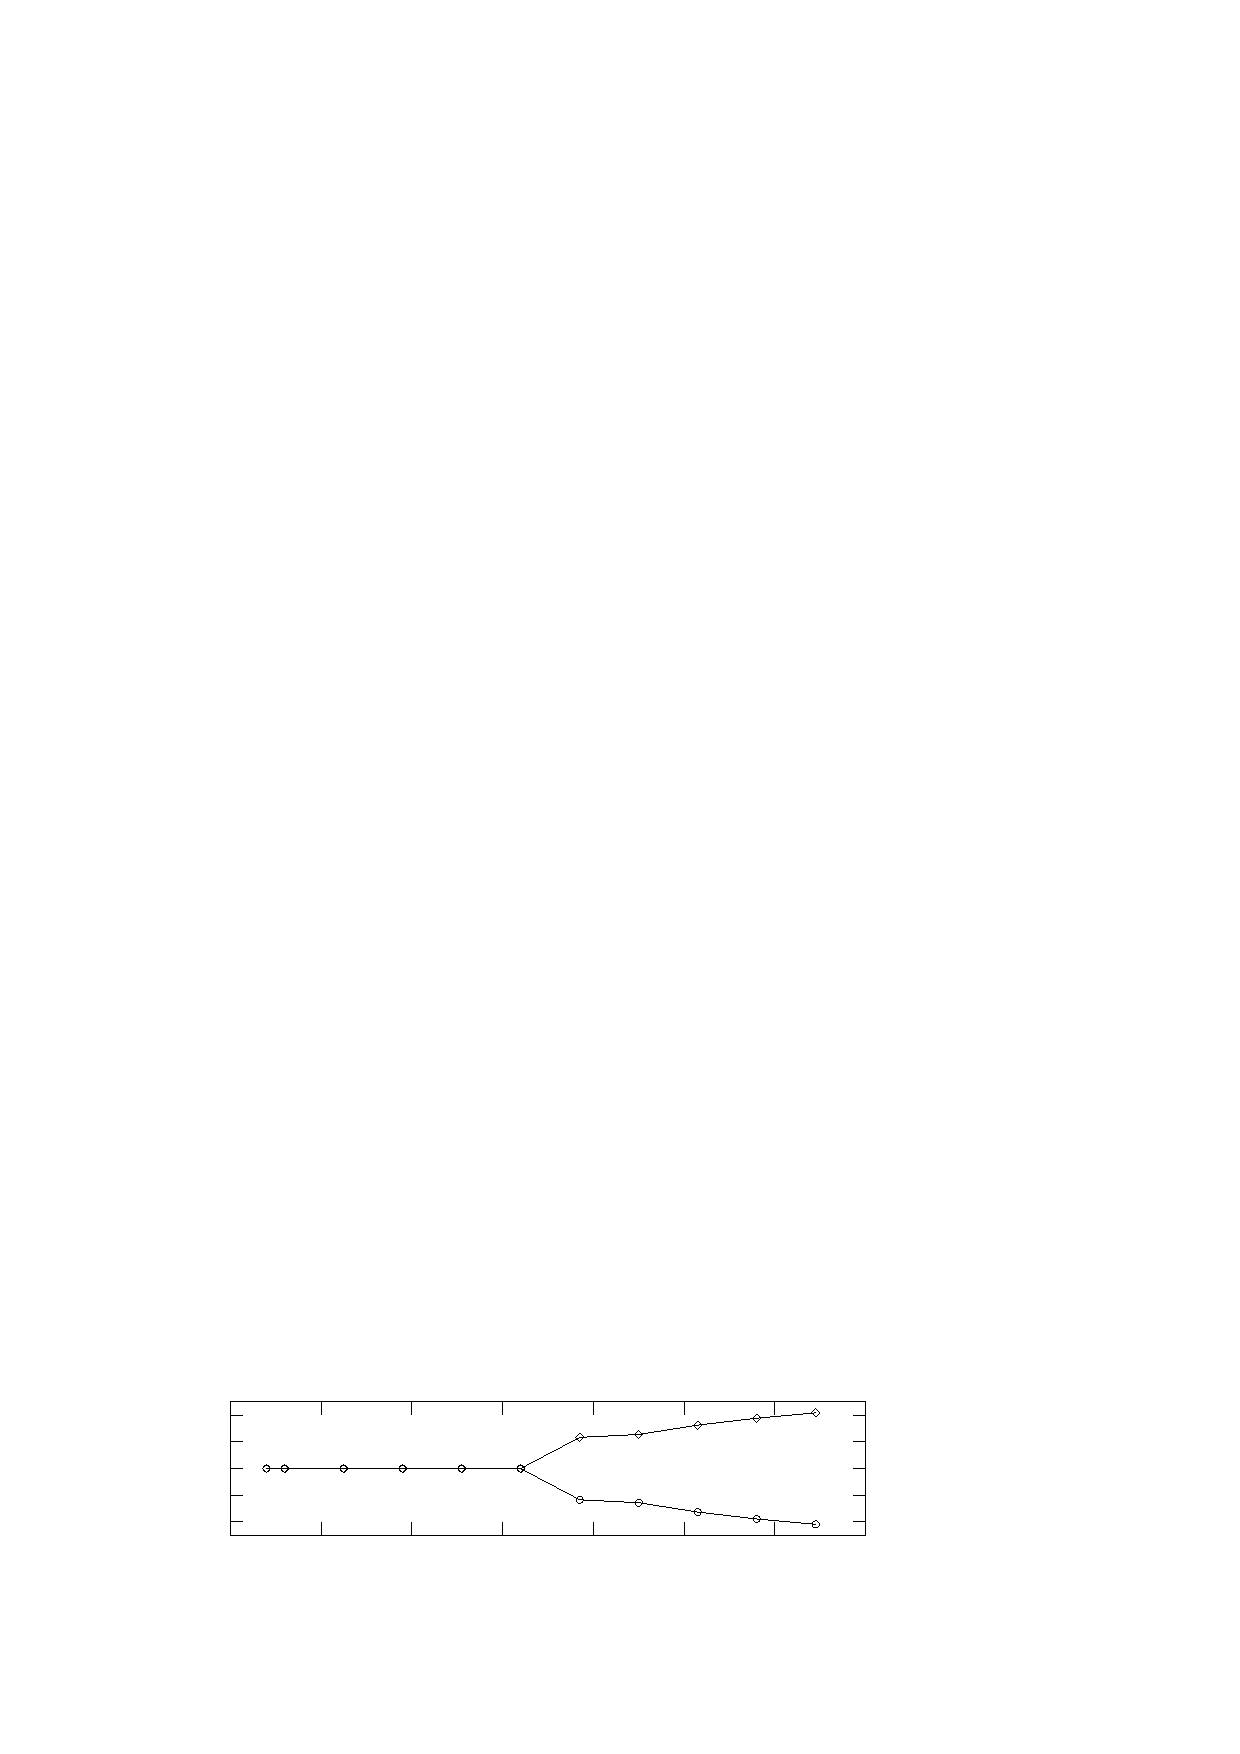
\includegraphics{bifurcacion-rounded}%
\end{picture}%
\begingroup
\setlength{\unitlength}{0.0200bp}%
\begin{picture}(18000,5400)(0,0)%
\put(1650,1970){\makebox(0,0)[r]{\strut{}-2}}%
\put(1650,2610){\makebox(0,0)[r]{\strut{}-1}}%
\put(1650,3250){\makebox(0,0)[r]{\strut{}0}}%
\put(1650,3890){\makebox(0,0)[r]{\strut{}1}}%
\put(1650,4530){\makebox(0,0)[r]{\strut{}2}}%
\put(1925,1100){\makebox(0,0){\strut{}0.000}}%
\put(4104,1100){\makebox(0,0){\strut{}0.001}}%
\put(6282,1100){\makebox(0,0){\strut{}0.002}}%
\put(8461,1100){\makebox(0,0){\strut{}0.003}}%
\put(10639,1100){\makebox(0,0){\strut{}0.004}}%
\put(12818,1100){\makebox(0,0){\strut{}0.005}}%
\put(14996,1100){\makebox(0,0){\strut{}0.006}}%
\put(17175,1100){\makebox(0,0){\strut{}0.007}}%
\put(550,3250){\rotatebox{90}{\makebox(0,0){\strut{}$x^\ast$}}}%
\put(9550,275){\makebox(0,0){\strut{}$P_o^\ast$}}%
\end{picture}%
\endgroup
\endinput

\caption{\label{fig:bifurcacion-rounded} Horizontal position of the pressure node 
 with $\rho_p/\rho_f=50$. We identify $P_{o_c}^\ast$ between 0.0032 and 0.0038.}
\end{figure}
%
\begin{figure}
%GNUPLOT: LaTeX picture with Postscript
\begin{picture}(0,0)%
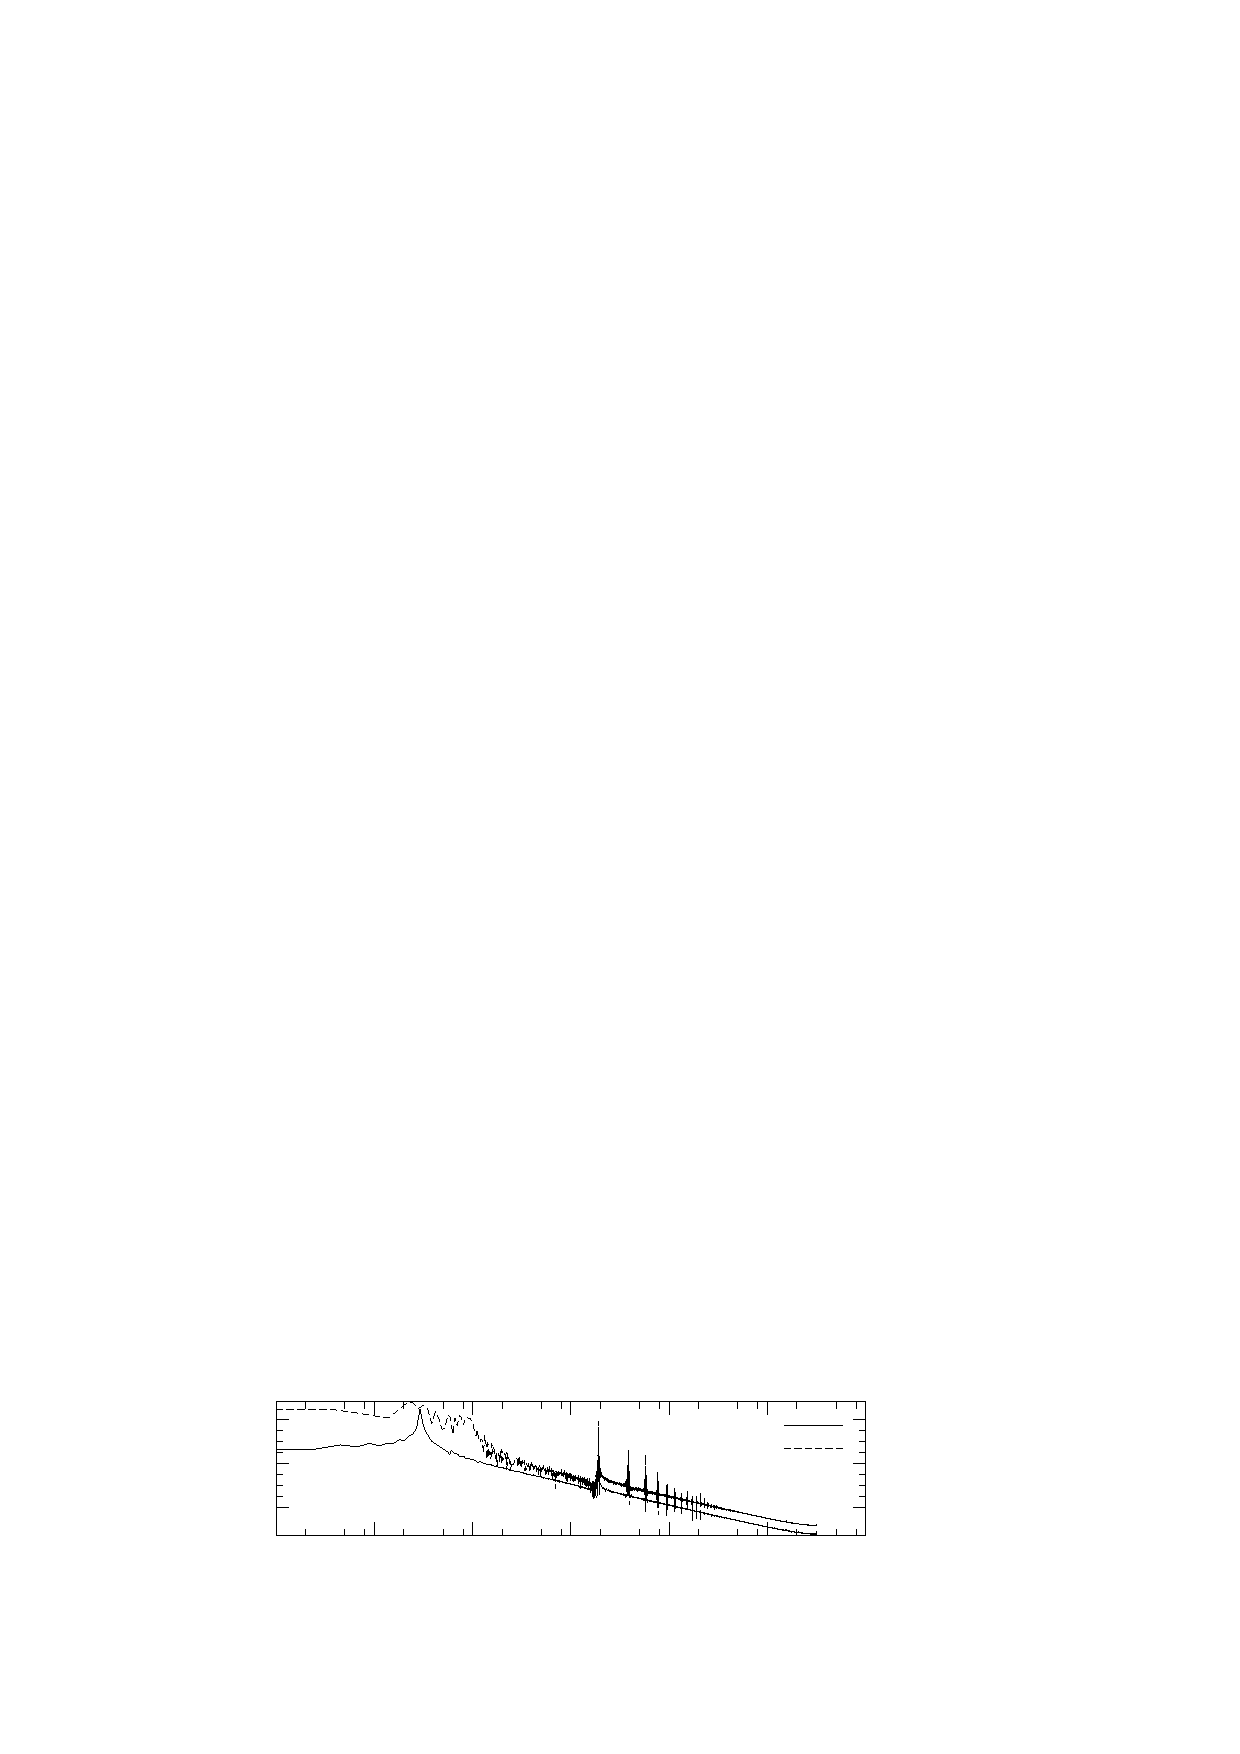
\includegraphics{figs/spectrums-rounded-first-last-Po}%
\end{picture}%
\begingroup
\setlength{\unitlength}{0.0200bp}%
\begin{picture}(18000,5400)(0,0)%
\put(2750,2318){\makebox(0,0)[r]{\strut{} 1e-12}}%
\put(2750,3379){\makebox(0,0)[r]{\strut{} 1e-08}}%
\put(2750,4440){\makebox(0,0)[r]{\strut{} 1e-04}}%
\put(3025,1100){\makebox(0,0){\strut{} 1e-05}}%
\put(5383,1100){\makebox(0,0){\strut{} 1e-04}}%
\put(7742,1100){\makebox(0,0){\strut{} 0.001}}%
\put(10100,1100){\makebox(0,0){\strut{} 0.01}}%
\put(12458,1100){\makebox(0,0){\strut{} 0.1}}%
\put(14817,1100){\makebox(0,0){\strut{} 1}}%
\put(17175,1100){\makebox(0,0){\strut{} 10}}%
\put(550,3250){\rotatebox{90}{\makebox(0,0){\strut{}PSD}}}%
\put(10100,275){\makebox(0,0){\strut{}$\omega$}}%
\put(14950,4275){\makebox(0,0)[r]{\strut{}$P_o^\ast = 6.00\times 10^{-4}$}}%
\put(14950,3725){\makebox(0,0)[r]{\strut{}$P_o^\ast = 6.45\times 10^{-3}$}}%
\end{picture}%
\endgroup
\endinput

\caption{ \label{fig:fig-spectrums-rounded-first-last-Po-1} Power spectra of the 
 vertical motion shown in Fig.~\ref{fig:paths-rho-30-rounded} (a), 
 continuous curve with $\omega_o =  0.019126$ and $\omega_1 = 0.0002913$ and
 the vertical motion shown in Fig.~\ref{fig:paths-rho-30-rounded} (c)
 with the same value of $\omega_o$.}
\end{figure}


%%%%%%%%%%%%%%%%%%%%%%%%%%%%%%%%%%%%%%%%%%%%%%%%%%%%%%%%%%%%%%%%%%%%%%%%%%%%%%%%%%%%%%%

\section{\label{sec:conclusions} Concluding remarks}

The lattice Boltzmann method can account for the interaction of a compressible fluid with a 
solid moving particle in acoustic levitation. We performed  numerical simulations when the 
ratio of densities of the particle and fluid varies for one fixed value of the momentum 
added by the acoustic source for the flat and rounded cavities. The average height at which 
the particle oscillates varies linearly with the density ratio for both cavities. 
The particle oscillates with the frequency of the acoustic source and its harmonics and in 
some cases with a much smaller frequency. When the momentum of the acoustic source varies 
for a fixed value of the density ratio, the particle in the flat cavity oscillates around 
a vertical position that approaches the pressure node as the momentum increases, again 
with the frequency of the acoustic source and its harmonics and in some cases with a 
smaller frequency. For the rounded cavity, the appearance of two pressure nodes destabilizes
the oscillation which may turn to be aperiodic due to the horizontal motion of the particle 
around the two pressure nodes. We speculate that the particle is the source of an 
asymmetric horizontal force that gives rise to such an aperiodic behaviour. We
could not find a chaotic motion but we did not explore the whole parameter space.

Altough we have focused on the motion of the particle, we can also focus on
the fluid. For example, we measured the streaming velocity defined as the time averaged 
velocity at a site and our results agree with those of~(\cite{haydock05b}, who found that the 
maximum streaming velocity is almost 2\% of the maximum velocity inside the cavity.

Using the LBM, simulations in complicated geometries can be carried out. These may  
help to determine the shift in the resonant frequency due to the presence of 
a particle and optimize the geometry of the reflector for a single or multiple 
axis levitator. 

%%%%%%%%%%%%%%%%%%%%%%%%%%%%%%%%%%%%%%%%%%%%%%%%%%%%%%%%%%%%%%%%%%%%%%%%%%%%%%%%%%%%%%%

\section*{Acknowledgments}

The authors thank Guadalupe Huelsz for suggesting the study of acoustic levitation and
proofreading the manuscript. The authors also thank H\'ector Cort\'es, Francisco Mandujano,
Eduardo Ramos, and Jorge Rojas for fruitful discussions and suggestions. Partial economic 
support from CONACyT project U41347 is acknowledged. G.~Barrios thanks CONACyT for a 
postgraduate scholarship. 
